% ============================================================
%  Hybrid PQ-OPAQUE — Full Journal Paper
%  Target template: Elsevier elsarticle (JISA-oriented draft)
%  Compiler: pdfLaTeX
% ============================================================
\documentclass[preprint,12pt]{elsarticle}
\biboptions{numbers}

% ── Language & Encoding (pdfLaTeX) ───────────────────────────
\usepackage[T1]{fontenc}
\usepackage[utf8]{inputenc}
\usepackage{lmodern}
\usepackage[english]{babel}
\usepackage{silence}
\WarningFilter{amsmath}{Unable to redefine math accent \vec}

% ── Mathematics ──────────────────────────────────────────────
\makeatletter
\let\vec\@undefined
\makeatother
\usepackage{amsmath}
\usepackage{amssymb}
\usepackage{amsthm}
\usepackage{mathtools}

% ── Tables ───────────────────────────────────────────────────
\usepackage{graphicx}
\usepackage{booktabs}
\usepackage{tabularx}
\usepackage{multirow}
\usepackage{array}
\usepackage{longtable}
\usepackage{makecell}
\usepackage{lscape}
\usepackage{tikz}
\usetikzlibrary{arrows.meta,positioning,shapes.geometric}

\usepackage{xcolor}
\definecolor{eclblue}{RGB}{27,74,139}
\definecolor{eclgold}{RGB}{217,136,29}
\definecolor{eclgreen}{RGB}{49,125,92}
\definecolor{eclred}{RGB}{171,67,53}

% ── Layout & Typography ──────────────────────────────────────
\emergencystretch=2em
\hfuzz=20pt
\hbadness=10000
\vbadness=10000
\raggedbottom
\setlength{\textfloatsep}{10pt plus 2pt minus 4pt}
\setlength{\floatsep}{8pt plus 2pt minus 2pt}
\setlength{\intextsep}{10pt plus 2pt minus 2pt}

% ── Hyperlinks ───────────────────────────────────────────────
\usepackage{hyperref}
\hypersetup{
  colorlinks=true,
  linkcolor=black,
  citecolor=black,
  urlcolor=blue,
}
\urlstyle{same}

% ── Custom column types ──────────────────────────────────────
\newcolumntype{L}[1]{>{\raggedright\arraybackslash}p{#1}}
\newcolumntype{C}[1]{>{\centering\arraybackslash}p{#1}}
\newcolumntype{R}[1]{>{\raggedleft\arraybackslash}p{#1}}
\newcommand{\acct}{\mathsf{acct}}
\newcommand{\sigoprf}{\sigma_{\mathrm{oprf}}}
\newcommand{\Label}[1]{L_{\mathrm{#1}}}
\newcommand{\KLabel}[1]{\Lambda_{\mathrm{#1}}}
\newcommand{\codeid}[1]{\textsf{#1}}

% ── Theorem environments ─────────────────────────────────────
\newtheorem{definition}{Definition}[section]
\newtheorem{theorem}{Theorem}[section]
\newtheorem{lemma}[theorem]{Lemma}
\newtheorem{proposition}[theorem]{Proposition}
\newtheorem{corollary}[theorem]{Corollary}
\theoremstyle{remark}
\newtheorem{remark}[theorem]{Remark}
\newtheorem{claim}[theorem]{Scoped security argument}
\newtheorem{example}[theorem]{Example}
\newtheorem{utheorem}{Theorem}
\newenvironment{sketchproof}{\par\noindent\textit{Proof sketch.}\ }{\par}

% ============================================================
\begin{document}
% ============================================================

\begin{frontmatter}

\title{Hybrid Post-Quantum Authentication from OPAQUE and ML-KEM-768: Construction, Formal Analysis, and a Reproducible Implementation}

\author[aff1]{Oleksandr Melnychenko}

\address[aff1]{Khmelnytskyi National University, Khmelnytskyi, Ukraine}

\journal{Journal of Information Security and Applications}

% ============================================================
\begin{abstract}
% ============================================================
Password-authenticated key exchange remains a practical authentication
mechanism, but classical OPAQUE relies on elliptic-curve hardness and has
no native post-quantum contribution in the authentication transcript. This
paper studies a narrower migration question: can an OPAQUE-like augmented
PAKE be reinforced with ML-KEM-768 while preserving the three-message
KE1--KE2--KE3 interaction profile and making the resulting syntax
independently auditable?

We specify Hybrid PQ-OPAQUE, a concrete OPAQUE-derived construction in
which four Ristretto255 Diffie--Hellman terms and one ML-KEM-768 shared
secret are combined by HKDF under a transcript-dependent salt. The
specification fixes the byte-level message layout, account-context binding
through $\acct$, deterministic derivation of the OPRF key from the service
root secret $\sigoprf$, and inclusion of $pk_{\mathrm{kem}}$ and
$ct_{\mathrm{kem}}$ in the authenticated transcript.

The evidence is deliberately scoped. ProVerif~2.05 models secrecy and
authentication in separate symbolic models; Tamarin~Prover~1.10.0 checks a
surrogate 4DH model; and the Rust artifact exercises serialization,
state-lifecycle, rejection, and benchmark paths. These results support a
bounded design argument rather than a machine-checked proof of the
implementation or a full computational proof of the hybrid combiner.

On the stated Linux/Xeon benchmark platform, the complete hybrid handshake
occupies 2715~bytes, end-to-end authentication takes 836.11~ms, and the
KSF-free post-quantum path adds 379.45~$\mu$s. The main performance
constraint is Argon2id rather than ML-KEM, while the main operational
boundary is separation of $\sigoprf$ from passive authentication records.
\end{abstract}

\begin{keyword}
OPAQUE \sep PAKE \sep ML-KEM-768 \sep post-quantum cryptography \sep hybrid key exchange \sep Ristretto255 \sep HKDF \sep Tamarin \sep ProVerif \sep Rust
\end{keyword}

\end{frontmatter}

% ============================================================
\section{Introduction}
% ============================================================

\subsection{Motivation}

Password authentication remains widely deployed in contemporary distributed systems. Survey evidence indicates that more than 80\% of authentication procedures in web applications and network services still rely on passwords~\cite{bonneau2012,florencio2007}. Password-authenticated key-exchange protocols (PAKEs) allow two parties sharing a low-entropy secret to establish a protected channel without revealing that secret to an adversary~\cite{bellare2000}. Among augmented PAKE constructions, OPAQUE~\cite{jarecki2018} is a well studied scheme: under compromise of the authentication database alone, the server stores a cryptographic record rather than a password equivalent~\cite{ietf-opaque}. In deployed systems, this property depends on a clear trust boundary, because compromise of the global secret from which OPRF keys are derived is distinct from compromise of a passive record store.

This reliance on classical hardness assumptions is a concern in the presence of quantum adversaries. Shor's algorithm~\cite{shor1994} applies to cryptosystems based on the discrete logarithm problem, including elliptic-curve key exchange and PAKE constructions built on related assumptions~\cite{bernstein2017}. Earlier estimates suggested that breaking Ristretto255/Curve25519 would require a cryptographically relevant quantum computer with approximately 2{,}330 logical qubits~\cite{roetteler2017}. More recent work reports two resource profiles for Shor's algorithm against 256-bit ECDLP over the \codeid{secp256k1} curve: no more than 1200 logical qubits with 90 million Toffoli operations, or no more than 1450 logical qubits with 70 million Toffoli operations~\cite{babbush2026}. These figures are not parameter-specific estimates for Ristretto255. They are used here only as a contemporary calibration point for 256-bit elliptic-curve migration risk. The store-now-decrypt-later strategy~\cite{mosca2018}, in which an adversary archives encrypted traffic for future decryption, adds to that motivation for systems protecting long-lived confidential data.

In August 2024, NIST published the first post-quantum cryptography standards, including FIPS~203 for ML-KEM~\cite{fips203} and FIPS~204 for ML-DSA~\cite{fips204}. Hybrid constructions that combine classical and post-quantum components are being introduced in TLS~1.3~\cite{stebila2024}, Signal (PQXDH)~\cite{brendel2020}, and WireGuard~\cite{hulsing2021}. Password authentication has not reached the same level of standardization. Classical OPAQUE in its current IETF specification~\cite{ietf-opaque} contains no mechanism aimed at quantum attacks, and other established PAKE protocols such as SRP and SPAKE2 have the same limitation. Recent work on post-quantum and hybrid PAKE has produced compact KEM-based constructions~\cite{arriaga2024}, UC/QROM-secure schemes~\cite{lyu2024uc}, and formal studies of hybrid composition~\cite{hesse2024,lyu2024hybrid}. What remains less developed is the combination of an augmented-PAKE design with explicit message syntax, scoped formal claims, measurements, and implementation-level evidence.

The concrete instantiation is anchored in final standards where such
standards exist: ML-KEM-768 follows FIPS~203~\cite{fips203}, OPAQUE is
compared against RFC~9807~\cite{ietf-opaque}, Ristretto255 follows
RFC~9496~\cite{devalence2024}, and HKDF follows RFC~5869~\cite{krawczyk2010}.
Argon2id~\cite{biryukov2016} is used as the password-hardening baseline,
and Criterion~\cite{heyer2023} is used only as the measurement framework
for the Rust artifact.

A secondary application motivation is audit-heavy cyber-physical
authentication, where login events may be part of telemetry, inspection,
and operational-control workflows rather than isolated web sessions
~\cite{svystun2025dytam,svystun2024thermal,lysyi2025fire}. These works
motivate stable protocol records and explicit failure semantics, but they
are not evidence for the cryptographic security of Hybrid PQ-OPAQUE.

\subsection{Research Scope and Evaluation Objective}

This paper studies a narrower engineering question: whether OPAQUE can be reinforced with ML-KEM-768 while preserving its three-message authentication flow. The construction combines four Ristretto255 Diffie--Hellman values with an ML-KEM-768 shared secret, fixes wire-format versioning, binds an explicit account context represented by the account identifier $\acct$ into the transcript, and evaluates the result using symbolic analysis and an executable reference implementation in Rust. The contribution is not a general theory of hybrid PAKE composition; it is an implementation-level augmented-PAKE design with explicit syntax, stated assumptions, and a deliberately limited claim set.

The evaluative objective is to determine whether this migration profile can be
specified, modeled, implemented, and measured without silently changing the
OPAQUE interaction profile or the augmented-PAKE trust boundary. The paper
therefore keeps each claim tied to a corresponding evidence layer, as
summarized in Table~\ref{tab:objective-evidence}. In this paper, the research
artifact denotes the accompanying source package that keeps these evidence
layers aligned: Rust crates, formal models, archived verification logs, tests,
benchmark harnesses, and adapter documentation.

\begin{table}[htbp]
\caption{Evaluation objective and evidence layers used in the manuscript}
\label{tab:objective-evidence}
\centering\scriptsize
\begin{tabularx}{\textwidth}{@{}L{3.2cm}L{5.2cm}X@{}}
\toprule
Question & Evidence used & Boundary \\
\midrule
Can ML-KEM be added without an extra message? & KE1--KE2--KE3 syntax,
wire-size accounting, and serializer tests & This is an OPAQUE-like
migration profile, not a claim of full RFC~9807 conformance. \\
Is the post-quantum material transcript-bound? & Account context,
extended transcript equations, MAC confirmation, and mutation tests &
The combiner argument is scoped to the stated extractor interpretation. \\
What formal evidence supports the design? & Split ProVerif models and a
surrogate Tamarin 4DH model & Symbolic evidence does not machine-check the
Rust implementation or side-channel behavior. \\
What is the measured cost? & Criterion benchmarks on the stated Linux/Xeon
platform & Timings are platform-specific and require recalibration on mobile,
browser, and embedded targets. \\
\bottomrule
\end{tabularx}
\end{table}

\subsection{Research Contributions}

\begin{enumerate}
  \item \textbf{A concrete OPAQUE migration profile.} The paper specifies a
        three-message OPAQUE-derived construction that combines four
        Ristretto255 DH terms with an ML-KEM-768 shared secret, fixes
        wire-format versioning, and binds account context,
        $pk_{\mathrm{kem}}$, and $ct_{\mathrm{kem}}$ into the
        authenticated transcript.
  \item \textbf{A scoped evidence package.} The manuscript aligns reduction
        sketches, two ProVerif models, a surrogate Tamarin 4DH model, and
        executable conformance tests to the same claim boundary, while
        explicitly separating symbolic evidence from implementation proof.
  \item \textbf{A reproducible cost and trust-boundary analysis.} The artifact
        reports message expansion, Criterion benchmarks, and operational
        assumptions for $\sigoprf$, showing that the dominant latency comes
        from Argon2id while the main new overhead is wire-format expansion.
\end{enumerate}

The remainder of the paper follows a claim-evidence structure.
Section~2 positions the construction against OPAQUE, post-quantum PAKE,
and hybrid-composition work. Section~3 states the objective, roles, assets,
and threat boundary. Section~4 specifies the protocol syntax and key
schedule. Section~5 states the symbolic security interpretation and its
limits. Section~6 reports measurements and then separates implementation
diagnostics from the main results.

\subsection{Terminology}

Table~\ref{tab:terminology} fixes the small vocabulary needed before the
protocol is defined. In particular, the distinction between payload and
wire format, and the role of $\acct$ as cryptographic context, are used
throughout the construction.

\begin{table}[htbp]
\caption{Terminology used in the paper}
\label{tab:terminology}
\centering\small
\begin{tabularx}{\textwidth}{@{}L{3.2cm}X@{}}
\toprule
Term & Meaning in this paper \\
\midrule
Wire format & The complete byte-level representation of a message on the channel, including the version prefix and protocol service fields \\
Payload & The message body excluding the version prefix and any external wrappers \\
Account identifier ($\acct$) & A stable byte string identifying the user's account; in this construction it is cryptographic context, not only a database lookup key \\
Initiator $\mathcal{C}$ & The party that holds the password, creates KE1, verifies KE2, and sends KE3 \\
Record-holding responder $\mathcal{S}$ & The augmented-PAKE party that stores the registration record, evaluates the OPRF, creates KE2, and verifies KE3 \\
Augmented PAKE (aPAKE) & A class of password-authenticated key-exchange protocols in which the server stores a verifier rather than the password itself or its direct equivalent \\
Key-derivation scheme & The sequence of extraction and expansion procedures that produces session and auxiliary keys \\
Research artifact & Source code, formal models, tests, and benchmarks needed for independent reproduction of the reported results \\
\bottomrule
\end{tabularx}
\end{table}

In addition, the formal exposition uses $\acct$ for the account
identifier and $\sigoprf$ for the root secret from which server-side
OPRF keys are derived. Literal ASCII domain-separation strings are
replaced below with the symbols $\Label{oprf}$, $\Label{seed}$,
$\Label{key}$, $\Label{ksf}$, $\Label{salt}$, $\Label{ctx}$,
$L_{\tau}$, and $\Label{comb}$; for the purposes of formal analysis,
their stability and mutual distinctness matter, whereas the concrete
textual representation of the implementation string does not.
For byte strings, $\operatorname{Trunc}_n(X)$ denotes the leftmost
$n$ octets of $X$.
Advantage expressions in the manuscript are scoped labels for the
argument being made, not theorem-level security definitions for an
independent PAKE family. When a bound is written below, it should be read
under the stated compromise model, primitive assumptions, and modeling
abstractions of that subsection.

% ============================================================
\section{Related Work and Existing Solutions}
% ============================================================

This section distinguishes source status because post-quantum
standardization is still moving. Final standards and RFCs, including
FIPS~203 and RFC~9807, are treated as normative anchors; peer-reviewed
papers are used for established PAKE and post-quantum results; ePrints
and Internet-Drafts are used as current but provisional evidence; and
technical white papers are used only for contextual calibration.

\subsection{Password-Authenticated Key-Exchange Protocols}

Password-authenticated key exchange (PAKE) refers to a class of protocols
that enables two parties sharing a low-entropy secret (a password) to
establish an authenticated session key resistant to offline dictionary
attacks~\cite{boyko2000}. PAKE protocols are commonly divided into two
categories:

\begin{itemize}
  \item \emph{Balanced PAKE}, in which both parties store equivalent
        password-derived representations. Representative examples are
        EKE~\cite{bellovin1992}, SPAKE2~\cite{ladd2023}, and
        CPace/AuCPace~\cite{haase2019}.
  \item \emph{Augmented PAKE (aPAKE)}, in which the server stores only a
        verifier rather than the password or its direct equivalent.
        Representative examples are SRP~\cite{wu1998},
        AuCPace~\cite{haase2019}, and OPAQUE~\cite{jarecki2018}.
\end{itemize}

\begin{table}[htbp]
\caption{Comparative characteristics of selected PAKE protocols}
\label{tab:pake-comparison}
\centering\scriptsize
\begin{tabularx}{\textwidth}{@{}L{3.5cm}>{\centering\arraybackslash}X>{\centering\arraybackslash}X>{\centering\arraybackslash}X>{\centering\arraybackslash}X@{}}
\toprule
Property & EKE & SRP & SPAKE2 & OPAQUE \\
\midrule
Type & Balanced & Augmented & Balanced & Augmented \\
Non-equivalent server record & No & Partial & No & Yes \\
Pre-computation resistance & No & No & No & Yes \\
Forward secrecy & Yes & Yes & Yes & Yes \\
Resistance to server-record compromise & No & Partial & No & In the passive-database model \\
Formal security proof & Ideal-cipher model & None & ROM & UC \\
Quantum resistance & No & No & No & No \\
\bottomrule
\end{tabularx}
\end{table}

In Table~\ref{tab:pake-comparison}, the OPAQUE entry regarding server
storage compromise should be read in the narrow but standard sense of
compromise of the authentication-record database alone. It does not
cover compromise of a global server secret from which OPRF keys may be
derived.

\subsection{OPAQUE: A Formal Overview}

OPAQUE~\cite{jarecki2018} consists of a registration phase and an
authentication phase, both built around an oblivious pseudorandom
function (OPRF). Standard IETF OPAQUE uses triple Diffie--Hellman
(3DH):
$dh_1 = sk_S \cdot PK_C$ (mutual authentication),
$dh_2 = sk_S \cdot E_C$,
$dh_3 = e_S \cdot PK_C$ (forward secrecy).
The construction analyzed here adds a fourth Diffie--Hellman term,
$dh_4 = e_S \cdot E_C$. This term binds the two ephemeral components
within a single transcript and, at the level of 4DH intuition, is
intended to complicate UKS-like substitutions; here it is treated as a
design rationale rather than as an independently proved property. In this
paper, ``4DH'' denotes these four Diffie--Hellman terms in the key
schedule, not a fourth authentication message; the message flow remains
KE1--KE2--KE3.
Baseline OPAQUE has been proved in the Universal Composability (UC)
model~\cite{canetti2001}.

\textbf{Oblivious pseudorandom function (OPRF).} The OPRF core uses a
hash-to-group map into Ristretto255~\cite{devalence2024}:
\begin{equation}
  \label{eq:oprf-core}
  \begin{aligned}
    \alpha &= r \cdot H'(\mathrm{ctx} \,\|\, x),\\
    \beta &= k \cdot \alpha,\\
    F_k(x) &= r^{-1} \cdot \beta,
  \end{aligned}
\end{equation}
where $r \xleftarrow{\$} \mathbb{Z}_q^*$ is a random initiator-side
blinding scalar, $k$ is the responder's OPRF key, and $\mathrm{ctx}$ is
the domain-separation context for the invocation.

\subsection{Post-Quantum Cryptography and the NIST 2024 Standards}

ML-KEM-768 is selected at NIST security level~3 (roughly aligned with
AES-192). Its parameters are $|pk| = 1184$~bytes,
$|ct| = 1088$~bytes, and $|ss| = 32$~bytes under IND-CCA2 security.
The abstraction is
\begin{equation}
  \mathrm{KeyGen}() \to (pk, sk);\quad
  \mathrm{Encaps}(pk) \to (ct, ss);\quad
  \mathrm{Decaps}(sk, ct) \to ss.
\end{equation}

\subsection{Rationale for Selecting ML-KEM-768}

The selection of ML-KEM-768 follows from the deployment constraints of
interactive password authentication. ML-KEM-512 offers smaller messages
and lower overhead, but it targets NIST level~1. ML-KEM-1024 provides a
higher nominal security level, but it also increases message size and
transport cost. For interactive password authentication, where the
protocol already includes a comparatively expensive KSF, the relevant
design criterion is the balance among cryptographic strength, message
size, and deployability.

ML-KEM-768 provides a middle operating point in that trade-off space.
Within the ML-KEM family it aligns NIST level~3 with the long-term
protection of account credentials and session secrets while avoiding
the larger transport burden imposed by ML-KEM-1024. Although
$pk_{\mathrm{kem}}$ and $ct_{\mathrm{kem}}$ enlarge
messages relative to classical OPAQUE, they do not render the protocol
unsuitable for interactive use.

\subsection{Design Alternatives Considered}

Several hybridization strategies are possible, and they lead to
different operational trade-offs. A purely transport-layer migration,
for example, can use a post-quantum or hybrid TLS key exchange while
leaving the application authentication protocol unchanged. That path is
attractive for deployment, but it does not make the password-authentication
transcript itself hybrid. Conversely, replacing the OPRF with a
post-quantum OPRF would address the password-randomization layer more
directly, but efficient and standardized post-quantum OPRFs are less
mature than ML-KEM-based key establishment. A third option is to store
long-lived post-quantum material in the registration record. This would
increase migration pressure on account state and would enlarge the
server-side record that operators must protect.

The construction studied here therefore adopts a narrower design: keep
the OPRF and envelope structure close to OPAQUE, add ML-KEM-768 only in
the ephemeral authentication path, and bind the resulting public KEM
values into the same transcript that authenticates the classical
exchange. This choice does not address every post-quantum PAKE problem,
but it gives a concrete migration point whose wire format,
implementation cost, and trust boundary can be measured.
Table~\ref{tab:design-alternatives} records the alternatives considered
and the reason for selecting the ephemeral ML-KEM path.

\begin{table}[htbp]
\caption{Hybridization strategies and their implications for this work}
\label{tab:design-alternatives}
\centering\scriptsize
\begin{tabularx}{\textwidth}{@{}L{3.2cm}L{4.5cm}X@{}}
\toprule
Strategy & Benefit & Limitation for the present objective \\
\midrule
Hybrid transport only & Minimal application changes when the surrounding
channel already supports post-quantum key exchange & The PAKE transcript
and application-level authentication state remain classical. \\
Post-quantum OPRF replacement & Targets the password-randomization layer
directly & Efficient post-quantum OPRF choices are less standardized and
would change the registration and envelope design more deeply. \\
Persistent PQ material in the record & Can attach post-quantum state to
the account itself & Enlarges long-lived account records and complicates
staged migration. \\
Separate PAKE and KEM composition & Keeps the classical PAKE largely
unchanged & Requires a separate composition argument and careful binding
to avoid treating two independent handshakes as one authenticated
exchange. \\
Ephemeral ML-KEM in the OPAQUE transcript & Preserves three messages,
keeps PQ material out of the registration record, and exposes concrete
wire-format costs & Leaves the OPRF layer classical and requires a
carefully scoped hybrid-combiner interpretation. \\
\bottomrule
\end{tabularx}
\end{table}

\subsection{Recent Approaches to Post-Quantum PAKE (2023--2026)}

Between 2023 and 2026, several research lines became relevant to
post-quantum PAKE and hybrid aPAKE design.

KEM-based schemes indicate that compact lattice-based PAKE is feasible.
A representative example is CHIC~\cite{arriaga2024}, which
combines a compact construction with a UC-security argument and
implementation-level evaluation. In parallel, UC- and QROM-oriented
results such as~\cite{lyu2024uc} strengthen compositional guarantees
for the post-quantum setting. These results are important, but they do
not directly resolve the migration problem for deployed OPAQUE-like
systems, where asymmetric initiator--responder roles, wire-format stability,
and compatibility with existing authentication workflows are central.

A second line of work considers replacement of classical OPRF
components and the compilation of KEM primitives into PAKE.
Lattice-based post-quantum OPRF constructions remain
more communication-intensive than elliptic-curve instantiations
~\cite{beguinet2023}, and generalized KEM-to-PAKE approaches require
careful treatment of ideal-cipher assumptions, hashing into public-key
spaces, and low-entropy secrets~\cite{arriaga2024}. By contrast,
isogeny-based approaches have lost practical relevance after the
Castryck--Decru attacks on SIDH-derived constructions
~\cite{castryck2023}.

Recent work also treats hybridization itself as a distinct design
problem. PAKE combiners~\cite{hesse2024} and UC analyses of hybrid
PAKE~\cite{lyu2024hybrid} primarily address proof structure and
composition, while the CFRG-related hybrid PAKE draft~\cite{vos2025}
indicates active standardization interest. The present work is narrower:
it is not a new UC-secure PAKE family and not a general combiner theorem.
Its novelty is an OPAQUE migration profile with explicit transcript
syntax, no additional authentication message, no persistent
post-quantum account state, a stated $\sigoprf$ trust boundary, and
reproducible implementation measurements.

Compared with CHIC and UC/QROM-oriented post-quantum PAKEs, the
construction prioritizes migration from an augmented OPAQUE setting
rather than a clean-slate PAKE design. Compared with PAKE-combiner work,
it provides concrete wire syntax and artifact evidence rather than a
general composition proof. Compared with transport-only hybridization, it
binds the post-quantum contribution inside the password-authentication
transcript itself.

% ============================================================
\section{Problem Statement}
% ============================================================

\subsection{Problem Formulation and Threat Model}

Let $\mathcal{C}$ be the \emph{initiator} and $\mathcal{S}$ be the
\emph{record-holding responder}. The initiator holds the password
$\mathrm{pwd}$ and completes OPRF finalization locally. The responder
stores the registration record $\mathrm{rec}$ and derives
account-specific OPRF keys from $\sigoprf$. This vocabulary is used
throughout the threat model, figures, symbolic models, and implementation
discussion; deployment terms such as client and server are treated only
as explanatory aliases. Let $\mathbb{G}$ denote the
prime-order Ristretto255 group of order~$q$ with generator~$g$.

\textbf{Assets to be protected:}
\begin{itemize}
  \item the password $\mathrm{pwd}$; the static keys $sk_C, sk_S$; the
        ephemeral keys $e_C, e_S, sk_{\mathrm{kem}}$;
  \item the registration record
        $\mathrm{rec} = (\mathrm{envelope}, pk_C)$;
  \item the session key $K_s$, the master key $K_m$, and the shared
        secret $ss_{\mathrm{kem}}$.
\end{itemize}

\textbf{Adversarial model.} Three adversarial classes are considered:
\begin{itemize}
  \item \emph{Classical adversary $\mathcal{A}_C$}: a
        probabilistic polynomial-time active man-in-the-middle capable
        of compromising server-side storage;
  \item \emph{Quantum adversary $\mathcal{A}_Q$}: an adversary modeled
        as capable of solving DLP/ECDLP via Shor's algorithm and pursuing a
        ``harvest now, decrypt later'' strategy;
  \item \emph{Composite adversary $\mathcal{A}_{CQ}$}: an active
        man-in-the-middle equipped with a quantum computational oracle.
\end{itemize}

\textbf{Threat-model boundary.} The adversary controls the network and
may record, replay, delay, drop, and modify protocol messages. The
database-compromise scenario gives the adversary the registration
record and associated public metadata, but not the operational secret
$\sigoprf$ from which account-specific OPRF keys are derived. The model
also permits post-session compromise of long-term static protocol keys
when discussing forward secrecy. It does not include
full endpoint compromise during an active session, malicious random
number generation, password-reset workflows, resource-exhaustion
denial-of-service analysis, or microarchitectural side channels. These
excluded cases are operationally important, but they require different
mechanisms from the protocol-level construction studied here.

Operationally, the database-only claim requires $\sigoprf$ to be managed
outside the password-record store and outside ordinary database backup,
analytics, and logging paths. A conforming deployment should keep
$\sigoprf$ in a KMS, HSM, or equivalent secret-management boundary;
limit derivation access to the authentication service; exclude plaintext
$\sigoprf$ from snapshots, crash dumps, and support bundles; audit
derivation calls; and define an incident procedure in which suspected
$\sigoprf$ exposure is treated as verifier compromise, requiring root
rotation, account re-enrolment or password reset, and temporary rate
tightening.
Table~\ref{tab:threat-boundary} makes this boundary explicit for the
main claims.

\begin{table}[htbp]
\caption{Threat-model boundary used for the main security claims}
\label{tab:threat-boundary}
\centering\small
\begin{tabularx}{\textwidth}{@{}L{3.4cm}L{4.6cm}X@{}}
\toprule
Scenario & Included in the claim & Boundary \\
\midrule
Active network attack & Full Dolev--Yao control of messages and
transcript manipulation & Does not model traffic analysis or
availability attacks. \\
Database disclosure & Registration record, stored public keys, and
protocol metadata may be exposed & Offline resistance assumes
$\sigoprf$ remains outside the compromised store. \\
Post-session key exposure & Long-term static keys may be compromised
after completion & Session-local ephemerals and ML-KEM decapsulation
state are assumed destroyed. \\
Quantum attack on classical DH & Classical DH terms may be treated as
recoverable in the long-term migration argument & The post-quantum
layer is then relied upon under the ML-KEM assumption. \\
Implementation behavior & Serialization, state lifecycle, version
handling, and external-adapter errors are checked by tests & Tests do not establish
absence of side channels or memory-safety bugs in external crates. \\
\bottomrule
\end{tabularx}
\end{table}

\begin{figure}[htbp]
\centering
\resizebox{0.96\textwidth}{!}{%
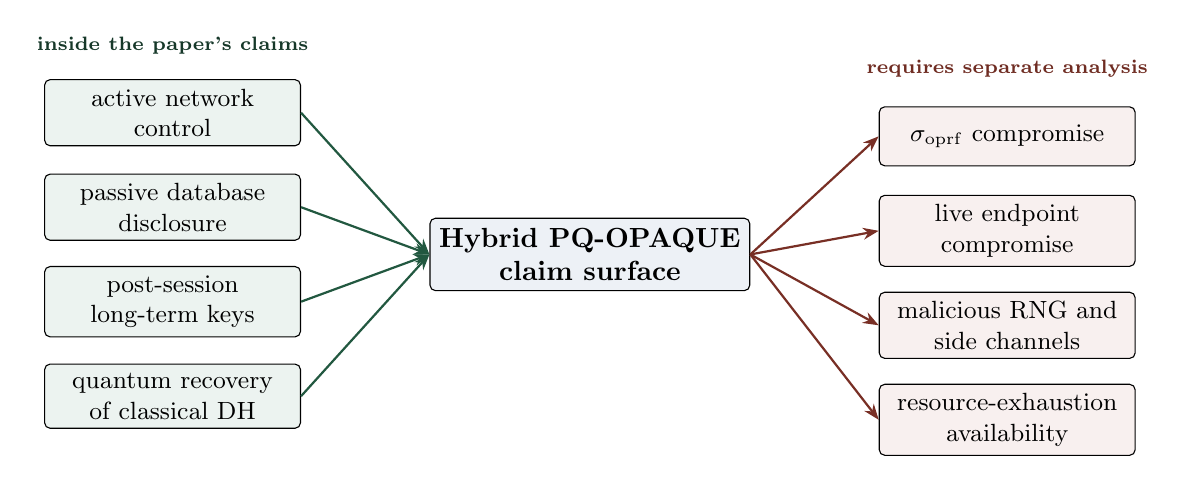
\begin{tikzpicture}[
  font=\small,
  >=Stealth,
  included/.style={draw,rounded corners=2pt,fill=eclgreen!9,
    minimum width=3.25cm,minimum height=0.75cm,align=center},
  excluded/.style={draw,rounded corners=2pt,fill=eclred!8,
    minimum width=3.25cm,minimum height=0.75cm,align=center},
  core/.style={draw,rounded corners=2pt,fill=eclblue!8,
    minimum width=3.65cm,minimum height=0.92cm,align=center,font=\bfseries},
  arrow/.style={-{Stealth[length=2mm]},thick}
]
  \node[core] (protocol) at (0,0) {Hybrid PQ-OPAQUE\\claim surface};

  \node[included] (network) at (-5.3,1.8) {active network\\control};
  \node[included] (database) at (-5.3,0.6) {passive database\\disclosure};
  \node[included] (ltkeys) at (-5.3,-0.6) {post-session\\long-term keys};
  \node[included] (quantum) at (-5.3,-1.8) {quantum recovery\\of classical DH};

  \node[excluded] (oprf) at (5.3,1.5) {$\sigoprf$ compromise};
  \node[excluded] (endpoint) at (5.3,0.3) {live endpoint\\compromise};
  \node[excluded] (rng) at (5.3,-0.9) {malicious RNG and\\side channels};
  \node[excluded] (dos) at (5.3,-2.1) {resource-exhaustion\\availability};

  \foreach \x in {network,database,ltkeys,quantum} {
    \draw[arrow,eclgreen!70!black] (\x.east) -- (protocol.west);
  }
  \foreach \x in {oprf,endpoint,rng,dos} {
    \draw[arrow,eclred!70!black] (protocol.east) -- (\x.west);
  }

  \node[anchor=south,font=\scriptsize\bfseries,text=eclgreen!45!black]
    at (-5.3,2.42) {inside the paper's claims};
  \node[anchor=south,font=\scriptsize\bfseries,text=eclred!65!black]
    at (5.3,2.12) {requires separate analysis};
\end{tikzpicture}
}
\caption{Threat-boundary map for the main claims. The construction is
analyzed against active network control, database disclosure, post-session
long-term key exposure, and later quantum recovery of classical DH terms.
Compromise of the OPRF root secret, live endpoint compromise, malicious
randomness, side channels, and availability attacks are outside the claim
surface.}
\label{fig:threat-boundary-map}
\end{figure}

\textbf{Protocol requirements:}
\begin{description}
  \item[R1] (OPAQUE-derived goals): password secrecy, forward secrecy,
        mutual authentication, and resistance to offline guessing;
  \item[R2] (Post-quantum reinforcement): inclusion of a KEM-based
        contribution against ``harvest now, decrypt later'' exposure;
  \item[R3] (Hybrid-source interpretation): the key-material combiner
        should support a stated extractor-based reading in the adopted
        model, so that the paper can identify precisely which source
        assumptions remain necessary for final-key recovery;
  \item[R4] (Interaction preservation): preservation of three protocol
        messages and 1.5 network round trips;
  \item[R5] (Implementability): a reproducible reference implementation
        in Rust suitable for further analysis and engineering.
\end{description}

\subsection{Formal Definitions}

\begin{definition}[KEM]
$(\mathrm{KeyGen}, \mathrm{Encaps}, \mathrm{Decaps})$:
$\mathrm{KeyGen}() \to (pk, sk)$;
$\mathrm{Encaps}(pk) \to (ct, ss)$;
$\mathrm{Decaps}(sk, ct) \to ss$.
IND-CCA2 security means that no polynomial-time adversary equipped with
a decapsulation oracle can distinguish the real $ss$ from a random
string.
\end{definition}

\begin{definition}[Hybrid aPAKE in the sense of this paper]
Protocol $\Pi$ between $\mathcal{C}(\mathrm{pwd})$ and
$\mathcal{S}(\mathrm{rec})$, in which
\[
  \begin{aligned}
    \mathrm{IKM}_{\mathrm{cl}}
      &= \operatorname{Encode}(dh_1) \| \operatorname{Encode}(dh_2)\\
      &\quad \| \operatorname{Encode}(dh_3) \|
        \operatorname{Encode}(dh_4),\\
    \mathrm{IKM}_{\mathrm{pq}} &= ss_{\mathrm{kem}},
  \end{aligned}
\]
and the final pre-key is formed as
\[
  \mathrm{PRK} = \mathrm{HKDF\text{-}Extract}\!\bigl(
    \mathrm{salt}_{\tau},\;
    \mathrm{IKM}_{\mathrm{cl}} \| \mathrm{IKM}_{\mathrm{pq}}\bigr).
\]
The subsequent analysis examines the extent to which such a
construction is compatible with the hybrid-source interpretation used
within the threat model considered here.
\end{definition}

\begin{definition}[Pseudorandomness of HKDF-Extract]
HKDF-Extract based on HMAC-SHA-512 is modeled as an extractor: if
$\mathrm{IKM}$ contains hidden computational entropy relative to the
adversary, then the output PRK is computationally indistinguishable
from uniform up to advantage at most~$\varepsilon$.
\end{definition}

\textbf{Notation:} $\mathbb{G}$ denotes Ristretto255 with
$|\mathbb{G}| = q$; lowercase letters denote scalars; uppercase letters
denote curve points; $\|$ denotes concatenation; $H(\cdot)$ denotes
SHA-512; and $\mathcal{K} = (K_s, K_m)$ denotes the session and master
keys.

% ============================================================
\section{The Proposed Hybrid PQ-OPAQUE Protocol}
% ============================================================

\subsection{Architecture and Overview}

Hybrid PQ-OPAQUE is a hybrid post-quantum extension of
OPAQUE~\cite{ietf-opaque}. The protocol preserves the augmented-PAKE
asymmetry: in an honest execution, the password is neither transmitted
to nor reconstructed by the record-holding responder. Authentication
remains a three-message KE1--KE2--KE3 exchange. The only post-quantum
state added to authentication is ephemeral ML-KEM-768 material:
$pk_{\mathrm{kem}}$ in KE1 and $ct_{\mathrm{kem}}$ in KE2.
Figure~\ref{fig:protocol-flow} shows where these values, together with
the account-context hash $\eta$, enter the transcript and key schedule.

\begin{figure}[htbp]
\centering
\resizebox{\textwidth}{!}{%
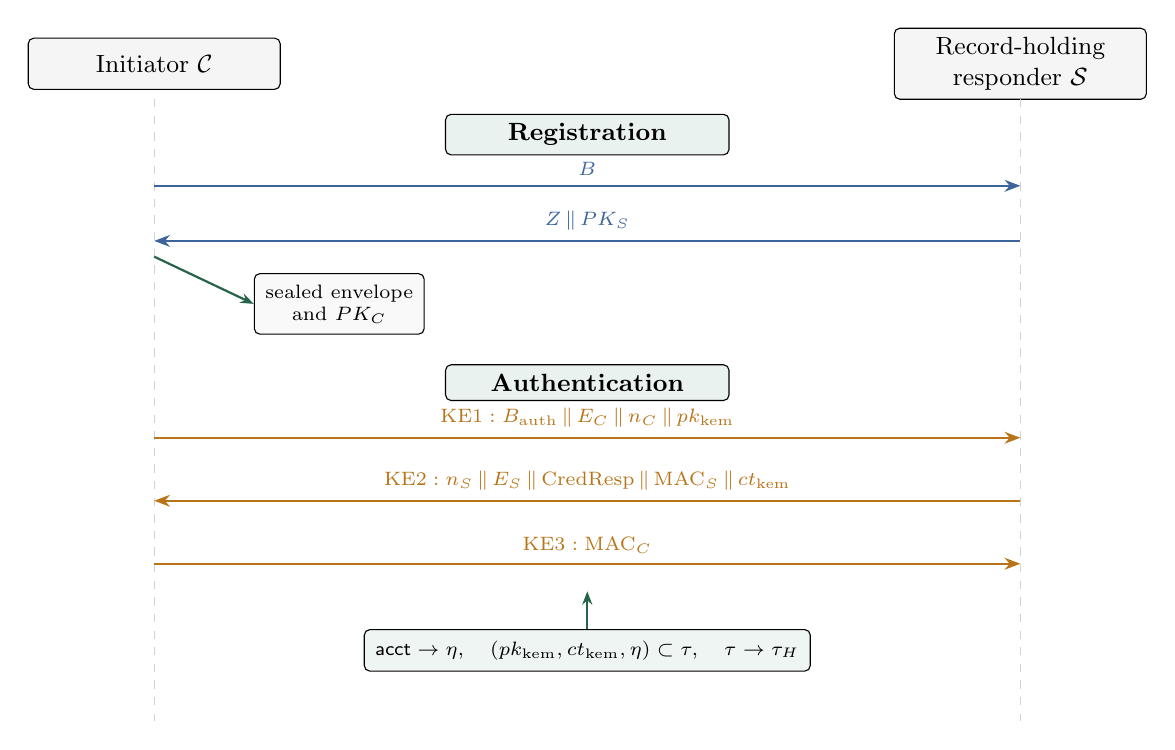
\begin{tikzpicture}[
  font=\small,
  >=Stealth,
  lane/.style={draw,rounded corners=2pt,fill=gray!8,minimum width=3.2cm,
    minimum height=0.65cm,align=center},
  phase/.style={draw,rounded corners=2pt,fill=eclgreen!10,minimum width=3.6cm,
    minimum height=0.45cm,align=center,font=\small\bfseries},
  note/.style={draw,rounded corners=2pt,fill=gray!5,align=center,
    inner sep=4pt,font=\scriptsize},
  msg/.style={-{Stealth[length=2mm]},thick},
  bind/.style={-{Stealth[length=1.7mm]},thick,eclgreen!80!black}
]
  \node[lane] (client) at (0,0) {Initiator $\mathcal{C}$};
  \node[lane] (server) at (11,0) {Record-holding\\responder $\mathcal{S}$};
  \draw[gray!35,dashed] (0,-0.45) -- (0,-8.35);
  \draw[gray!35,dashed] (11,-0.45) -- (11,-8.35);

  \node[phase] at (5.5,-0.9) {Registration};
  \draw[msg,eclblue!85] (0,-1.55) -- node[above,font=\scriptsize]
    {$B$} (11,-1.55);
  \draw[msg,eclblue!85] (11,-2.25) -- node[above,font=\scriptsize]
    {$Z \,\|\, PK_S$} (0,-2.25);
  \node[note] (record) at (2.35,-3.05)
    {sealed envelope\\and $PK_C$};
  \draw[bind] (0,-2.45) -- (record.west);

  \node[phase] at (5.5,-4.05) {Authentication};
  \draw[msg,eclgold!85!black] (0,-4.75) -- node[above,font=\scriptsize]
    {$\mathrm{KE1}: B_{\mathrm{auth}} \,\|\, E_C \,\|\, n_C \,\|\, pk_{\mathrm{kem}}$}
    (11,-4.75);
  \draw[msg,eclgold!85!black] (11,-5.55) -- node[above,font=\scriptsize]
    {$\mathrm{KE2}: n_S \,\|\, E_S \,\|\, \mathrm{CredResp}
      \,\|\, \mathrm{MAC}_S \,\|\, ct_{\mathrm{kem}}$}
    (0,-5.55);
  \draw[msg,eclgold!85!black] (0,-6.35) -- node[above,font=\scriptsize]
    {$\mathrm{KE3}: \mathrm{MAC}_C$}
    (11,-6.35);

  \node[note,fill=eclgreen!8] (acctnote) at (5.5,-7.45)
    {$\acct \rightarrow \eta,\quad
     (pk_{\mathrm{kem}},ct_{\mathrm{kem}},\eta) \subset \tau,\quad
     \tau \rightarrow \tau_H$};
  \draw[bind] (acctnote.north) -- (5.5,-6.70);
\end{tikzpicture}
}
\caption{Hybrid PQ-OPAQUE message flow between initiator $\mathcal{C}$
and record-holding responder $\mathcal{S}$. ML-KEM public and ciphertext
material are carried in KE1 and KE2, while account and transcript binding
feed the authenticated key schedule without adding an authentication
message.}
\label{fig:protocol-flow}
\end{figure}

Table~\ref{tab:primitives} fixes the concrete primitive choices used by
the construction and by the implementation evaluated below.

\begin{table}[htbp]
\caption{Cryptographic primitives used in Hybrid PQ-OPAQUE}
\label{tab:primitives}
\centering\small
\begin{tabular*}{\textwidth}{@{\extracolsep{\fill}}L{3.2cm}L{3.2cm}L{2.8cm}L{2cm}@{}}
\toprule
Component & Primitive & Implementation & Security level \\
\midrule
OPRF group & Ristretto255 & \makecell[l]{\codeid{curve25519-}\\\codeid{dalek}} & 128 bits \\
Hash function & SHA-512 & \codeid{sha2} & 256 bits \\
KDF (extract) & HKDF-Extract (HMAC-SHA-512) & \codeid{hmac + sha2} & 256 bits \\
KDF (expand) & HKDF-Expand (HMAC-SHA-512) & \codeid{hmac + sha2} & 256 bits \\
MAC & HMAC-SHA-512 & \codeid{hmac + sha2} & 256 bits \\
KSF & Argon2id (MODERATE) & \codeid{argon2} & Adaptive \\
AEAD & XSalsa20-Poly1305 & \makecell[l]{\codeid{crypto\_}\\\codeid{secretbox}} & 256 bits \\
KEM & ML-KEM-768 (FIPS~203) & \codeid{ml-kem} & NIST Level~3 \\
Classical exchange & 4DH (Ristretto255) & \makecell[l]{\codeid{curve25519-}\\\codeid{dalek}} & 128 bits \\
Constant-time comparison & Bytewise without early exit & \codeid{subtle} & --- \\
\bottomrule
\end{tabular*}
\end{table}

The authentication-message sizes in Table~\ref{tab:message-sizes}
separate payload size from wire-format size; the latter includes the
one-byte protocol version prefix.

\begin{table}[htbp]
\caption{Authentication-message sizes in payload and wire format}
\label{tab:message-sizes}
\centering\small
\resizebox{\textwidth}{!}{%
\begin{tabular}{lrrrr}
\toprule
Message & Classical payload & Hybrid payload & Hybrid wire format & Post-quantum overhead \\
\midrule
KE1 & 88 bytes & 1272 bytes & 1273 bytes & $+1184$ ($pk_{\mathrm{kem}}$) \\
KE2 & 288 bytes & 1376 bytes & 1377 bytes & $+1088$ ($ct_{\mathrm{kem}}$) \\
KE3 & 64 bytes & 64 bytes & 65 bytes & $0$ \\
\midrule
\textbf{Total} & \textbf{440 bytes} & \textbf{2712 bytes} & \textbf{2715 bytes} & \textbf{$+2272$ ($+516\%$)} \\
\bottomrule
\end{tabular}
}
\end{table}

\begin{figure}[htbp]
\centering
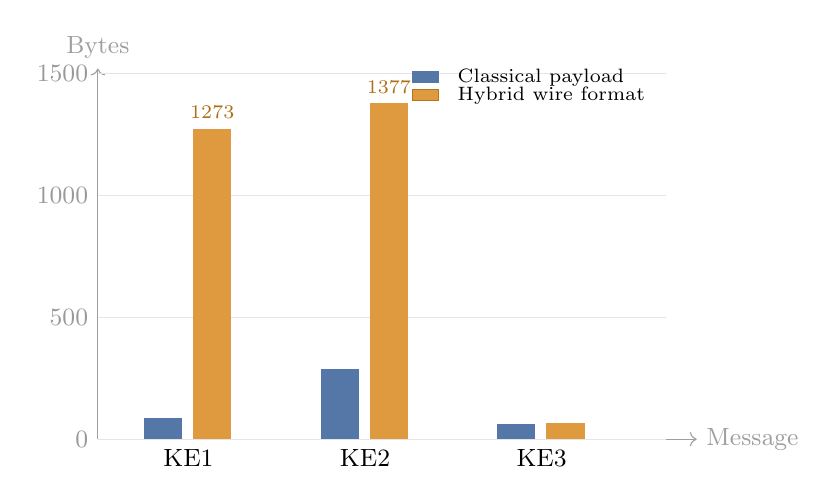
\begin{tikzpicture}[x=1.95cm,y=0.0031cm,font=\small]
  \draw[->,gray!75] (0,0) -- (3.9,0) node[right] {Message};
  \draw[->,gray!75] (0,0) -- (0,1520) node[above] {Bytes};

  \foreach \yy in {0,500,1000,1500} {
    \draw[gray!20] (0,\yy) -- (3.7,\yy);
    \node[left,gray!80] at (0,\yy) {\yy};
  }

  % KE1
  \fill[eclblue!75] (0.30,0) rectangle (0.55,88);
  \fill[eclgold!85] (0.62,0) rectangle (0.87,1273);
  \node[above,font=\scriptsize,eclgold!80!black] at (0.745,1273) {1273};
  \node[below] at (0.59,0) {KE1};

  % KE2
  \fill[eclblue!75] (1.45,0) rectangle (1.70,288);
  \fill[eclgold!85] (1.77,0) rectangle (2.02,1377);
  \node[above,font=\scriptsize,eclgold!80!black] at (1.895,1377) {1377};
  \node[below] at (1.74,0) {KE2};

  % KE3
  \fill[eclblue!75] (2.60,0) rectangle (2.85,64);
  \fill[eclgold!85] (2.92,0) rectangle (3.17,65);
  \node[below] at (2.89,0) {KE3};

  \draw[eclblue!75,fill=eclblue!75] (2.05,1462) rectangle (2.22,1507);
  \node[anchor=west,font=\scriptsize] at (2.28,1484) {Classical payload};
  \draw[eclgold!85!black,fill=eclgold!85] (2.05,1388) rectangle (2.22,1433);
  \node[anchor=west,font=\scriptsize] at (2.28,1410) {Hybrid wire format};
\end{tikzpicture}
\caption{Comparison of authentication-message sizes: the additional
wire-format overhead is concentrated in KE1 and KE2, whereas KE3
remains essentially unchanged.}
\label{fig:wire-size-growth}
\end{figure}

Figure~\ref{fig:wire-size-growth} shows that the post-quantum layer
leaves finalization almost unchanged while increasing the transport
budget of the first two messages, namely the phases that carry
$pk_{\mathrm{kem}}$ and $ct_{\mathrm{kem}}$.

\subsection{Normative Wire Format and Rejection Rules}
\label{sec:normative-wire}

All authentication messages are fixed-width byte strings. The first byte
is the protocol version $v=\mathtt{0x01}$. KE1, KE2, and KE3 contain no
endian-sensitive integer fields; all components below are copied exactly
as octet strings at fixed offsets. The account identifier $\acct$ is an
external authenticated-context input, not a field inside these messages.

\begin{table}[htbp]
\caption{Fixed authentication-message layout}
\label{tab:auth-wire-layout}
\centering\scriptsize
\begin{tabularx}{\textwidth}{@{}L{1.6cm}L{2.4cm}L{3.0cm}X@{}}
\toprule
Message & Offset range & Field & Length and validation rule \\
\midrule
KE1 & 0 & $v$ & 1 byte; must equal \texttt{0x01} \\
KE1 & 1--32 & $B_{\mathrm{auth}}$ & 32-byte blinded OPRF group element; canonical Ristretto encoding required \\
KE1 & 33--64 & $E_C$ & 32-byte initiator ephemeral Ristretto public key \\
KE1 & 65--88 & $n_C$ & 24-byte initiator nonce \\
KE1 & 89--1272 & $pk_{\mathrm{kem}}$ & 1184-byte ML-KEM-768 public key \\
\midrule
KE2 & 0 & $v$ & 1 byte; must equal \texttt{0x01} \\
KE2 & 1--24 & $n_S$ & 24-byte responder nonce \\
KE2 & 25--56 & $E_S$ & 32-byte responder ephemeral Ristretto public key \\
KE2 & 57--224 & $\mathrm{CredResp}$ & 168-byte credential response \\
KE2 & 225--288 & $\mathrm{MAC}_S$ & 64-byte HMAC-SHA-512 confirmation token \\
KE2 & 289--1376 & $ct_{\mathrm{kem}}$ & 1088-byte ML-KEM-768 ciphertext \\
\midrule
KE3 & 0 & $v$ & 1 byte; must equal \texttt{0x01} \\
KE3 & 1--64 & $\mathrm{MAC}_C$ & 64-byte HMAC-SHA-512 confirmation token \\
\bottomrule
\end{tabularx}
\end{table}

Parsing is fail-closed. Exact length is required before field
interpretation. Unsupported version is distinguished from malformed
length at the public API boundary, while MAC, envelope, and password
failures are collapsed into authentication failure to reduce account and
stage fingerprinting. Ristretto encodings must decompress canonically;
ML-KEM public keys and ciphertexts must have the FIPS~203 lengths shown
in Table~\ref{tab:auth-wire-layout}; malformed public inputs are rejected
rather than silently normalized.

\subsection{Registration Phase}

\textbf{Step~1 ($\mathcal{C} \to \mathcal{S}$).} Generation of the
static pair $(sk_C, PK_C)$ followed by OPRF blinding:
\begin{equation}
  r \xleftarrow{\$} \mathbb{Z}_q^*, \qquad
  B = r \cdot H'\!\bigl(\Label{oprf} \| \mathtt{0x00} \| \mathrm{pwd}\bigr).
  \label{eq:reg-blind}
\end{equation}
$\mathrm{RegistrationRequest} = B$ (32~bytes).

\textbf{Step~2 ($\mathcal{S} \to \mathcal{C}$).} Derivation of the OPRF
key:
\begin{align}
  s_{\mathrm{oprf}}
    &= \operatorname{Trunc}_{32}\!\left(
      \mathrm{HMAC}\!\bigl(\sigoprf, \Label{seed}\bigr)\right),
    \label{eq:oprf-seed}\\
  k_{\mathrm{oprf}}
    &= \mathrm{ScalarReduce}\!\bigl(
      \mathrm{HMAC}\!\bigl(
        s_{\mathrm{oprf}},\;
        \Label{key} \| \acct \| \mathrm{ctr}
      \bigr)\bigr),
    \label{eq:oprf-key}
\end{align}
where $\mathrm{ctr}$ is the smallest one-byte counter for which the resulting
scalar is non-zero. The responder computes
$Z = k_{\mathrm{oprf}} \cdot B$; the key $k_{\mathrm{oprf}}$ is then
immediately destroyed. The response is
$Z \| PK_S$ (64~bytes).

\textbf{Step~3 ($\mathcal{C}$).} OPRF unblinding:
\[
  U = r^{-1} \cdot Z.
\]
OPRF output:
\begin{equation}
  y_{\mathrm{oprf}} = H\!\bigl(\Label{oprf} \|
    \mathtt{0x01} \| \mathrm{pwd} \| U\bigr).
  \label{eq:oprf-output}
\end{equation}
KSF input and salt:
\begin{align}
  x_{\mathrm{ksf}}
    &= H\!\bigl(\Label{ksf} \|
      y_{\mathrm{oprf}} \| \mathrm{pwd}\bigr),\\
  \mathrm{salt}_{\mathrm{ksf}}
    &= \operatorname{Trunc}_{16}\!\left(
      H\!\bigl(\Label{salt} \| y_{\mathrm{oprf}}\bigr)\right).
\end{align}
The randomized password is then computed with Argon2id~\cite{biryukov2016}
as
\begin{equation}
  \mathrm{rwd} = \mathrm{Argon2id}\!\bigl(
    x_{\mathrm{ksf}},\; \mathrm{salt}_{\mathrm{ksf}};\;
    m = 256~\mathrm{MiB},\; t = 3,\; p = 1\bigr).
  \label{eq:rwd}
\end{equation}
The MODERATE profile is the reference benchmark profile, not a universal
protocol constant. It targets server-class, desktop, and B2B deployments
where approximately 256~MiB of memory per authentication attempt is
acceptable. Constrained clients should recalibrate the KSF profile and
must not inherit the statement that ML-KEM overhead is practically
negligible without remeasurement.

\begin{table}[htbp]
\caption{KSF profiles and benchmark status}
\label{tab:ksf-profiles}
\centering\small
\begin{tabularx}{\textwidth}{@{}L{2.4cm}L{3.3cm}L{3.0cm}X@{}}
\toprule
Profile & Parameters & Measured here? & Intended use \\
\midrule
LIGHT & $m=64$~MiB, $t=2$, $p=1$ & No & Constrained or latency-sensitive clients requiring separate calibration \\
MODERATE & $m=256$~MiB, $t=3$, $p=1$ & Yes & Reference server-class and desktop/B2B profile used for the reported measurements \\
HARD & $m\geq512$~MiB, $t\geq3$, $p=1$ & No & High-value accounts or environments where memory cost is acceptable \\
\bottomrule
\end{tabularx}
\end{table}
The envelope is sealed using XSalsa20-Poly1305 and a key derived via
HKDF;
$\mathrm{RegistrationRecord} = \mathrm{Envelope} \| PK_C$
(168~bytes of payload and 169~bytes in wire format, including the
version prefix).

\subsection{Binding of Account Identifier and Context}

The protocol fixes additional context that remains implicit in many
abstract descriptions of OPAQUE. Every wire-format message carries a
one-byte version prefix $v = \mathtt{0x01}$, which separates the
payload from the full transmission format and enables rejection of
unsupported versions. The protocol also uses an explicit account
identifier $\acct$, a stable byte string naming the account, treated not
merely as a database lookup key but as cryptographic context.

Define the account-context hash used by the evaluated artifact as a
domain-separated binding of the account identifier:
\begin{equation}
  \eta =
  H\!\bigl(
    \Label{ctx} \,\|\, \acct
  \bigr).
  \label{eq:acct-context}
\end{equation}
Here $\acct$ is supplied as a separate API input, is rejected if empty,
and is not serialized inside KE1, KE2, or KE3. The version byte $v$ is
validated at the wire-format layer rather than mixed into $\eta$ in the
current artifact. A future interoperability profile could make this
binding length-prefixed and version-indexed, but that would be a new
wire-compatible profile decision rather than a claim about the evaluated
implementation.
Distinct domain-separation labels separate the baseline OPRF, KSF, and
transcript contexts from the added account-binding and hybrid-combiner
contexts. The version indices embedded in these labels are local domain
identifiers rather than global version numbers of the overall scheme.
The identifier $\acct$ influences the protocol at two points:
\begin{enumerate}
  \item through derivation of an account-specific OPRF key, as in
        Eq.~\eqref{eq:oprf-key};
  \item through inclusion of $\eta$, defined in
        Eq.~\eqref{eq:acct-context}, in the extended transcript
        \eqref{eq:hybrid-transcript}, and hence in the hybrid combiner
        \eqref{eq:hybrid-prk} and the derived keys
        \eqref{eq:key-derivation}.
\end{enumerate}
This binding makes cross-account transplantation visible in transcript
verification even when the password is identical, and it makes the role
of account identity explicit in the cryptographic specification.

\subsection{Authentication Phase and Hybrid Key Exchange}

\subsubsection{Generation of KE1 from Initiator to Record-Holding Responder}

The initiator first samples the OPAQUE authentication randomness and creates
the ephemeral ML-KEM key pair advertised in the first message:
\begin{equation}
  \label{eq:ke1-generation}
  \begin{alignedat}{2}
    r_{\mathrm{auth}} &\xleftarrow{\$} \mathbb{Z}_q^*,        &\qquad
    B_{\mathrm{auth}}
      &= r_{\mathrm{auth}} \cdot
        H'\!\bigl(\Label{oprf} \| \mathtt{0x00} \| \mathrm{pwd}\bigr),\\
    e_C &\xleftarrow{\$} \mathbb{Z}_q^*,        &\qquad
    E_C &= e_C \cdot g,\\
    n_C &\xleftarrow{\$} \{0,1\}^{192},         &\qquad
    (pk_{\mathrm{kem}},sk_{\mathrm{kem}})
        &\leftarrow \mathrm{ML\text{-}KEM\text{-}768.KeyGen}().
  \end{alignedat}
\end{equation}
The resulting first authentication message is
\begin{equation}
  \label{eq:ke1-wire-format}
  \begin{aligned}
    \mathrm{KE1}
      &= B_{\mathrm{auth}} \,\|\, E_C \,\|\, n_C \,\|\, pk_{\mathrm{kem}},\\
    |\mathrm{KE1}|
      &= 32 + 32 + 24 + 1184
       = 1272~\text{bytes}.
  \end{aligned}
\end{equation}
With the one-byte protocol version prefix, the wire message
$v \,\|\, \mathrm{KE1}$ occupies 1273~bytes.
The value $B_{\mathrm{auth}}$ is a fresh authentication-phase OPRF
blinding value and is independent of the registration-phase value $B$ in
Eq.~\eqref{eq:reg-blind}. In the implementation API and wire parser,
this same 32-byte field is named \codeid{credential\_request}.

\subsubsection{Generation of KE2 from Record-Holding Responder to Initiator}

\textbf{Responder ephemeral material:}
\begin{equation}
  \label{eq:ke2-ephemeral-generation}
  e_S \xleftarrow{\$} \mathbb{Z}_q^*,\qquad
  E_S = e_S \cdot g,\qquad
  n_S \xleftarrow{\$} \{0,1\}^{192}.
\end{equation}

\textbf{Four-way Diffie--Hellman (4DH):}
\begin{equation}
  dh_1 = sk_S \cdot PK_C,\quad
  dh_2 = sk_S \cdot E_C,\quad
  dh_3 = e_S \cdot PK_C,\quad
  dh_4 = e_S \cdot E_C.
\end{equation}

\textbf{ML-KEM-768 encapsulation:}
\begin{equation}
  (ct_{\mathrm{kem}}, ss_{\mathrm{kem}})
    \leftarrow \mathrm{ML\text{-}KEM\text{-}768.Encaps}(pk_{\mathrm{kem}}).
\end{equation}

\textbf{Extended transcript} (including post-quantum elements):
\begin{align}
  \tau &= E_C \,\|\, E_S \,\|\, n_C \,\|\, n_S
         \,\|\, PK_C \,\|\, PK_S \,\|\,
         \mathrm{CredResp} \,\|\, pk_{\mathrm{kem}}
         \,\|\, ct_{\mathrm{kem}} \,\|\, \eta,
         \notag\\
  \tau_H &= H\!\bigl(L_{\tau} \| \tau\bigr).
  \label{eq:hybrid-transcript}
\end{align}

\textbf{Hybrid combiner:}
\begin{align}
  \mathrm{IKM}_{\mathrm{cl}}
    &= \operatorname{Encode}(dh_1) \| \operatorname{Encode}(dh_2)
       \| \operatorname{Encode}(dh_3) \| \operatorname{Encode}(dh_4),
  \notag\\
  \mathrm{IKM}_{\mathrm{pq}} &= ss_{\mathrm{kem}},
  \notag\\
  \mathrm{IKM}_{\mathrm{hyb}} &= \mathrm{IKM}_{\mathrm{cl}} \|
    \mathrm{IKM}_{\mathrm{pq}}
    \quad(128 + 32 = 160~\text{bytes}),
  \notag\\
  \mathrm{salt}_{\tau} &= \Label{comb} \| \tau_H,
  \notag\\
  \mathrm{PRK} &= \mathrm{HKDF\text{-}Extract}(\mathrm{salt}_{\tau},
    \mathrm{IKM}_{\mathrm{hyb}}).
  \label{eq:hybrid-prk}
\end{align}

Figure~\ref{fig:hybrid-key-schedule} shows the resulting dataflow from
the classical 4DH terms, the ML-KEM shared secret, and the transcript
hash into the derived session keys.

\begin{figure}[htbp]
\centering
\resizebox{\textwidth}{!}{%
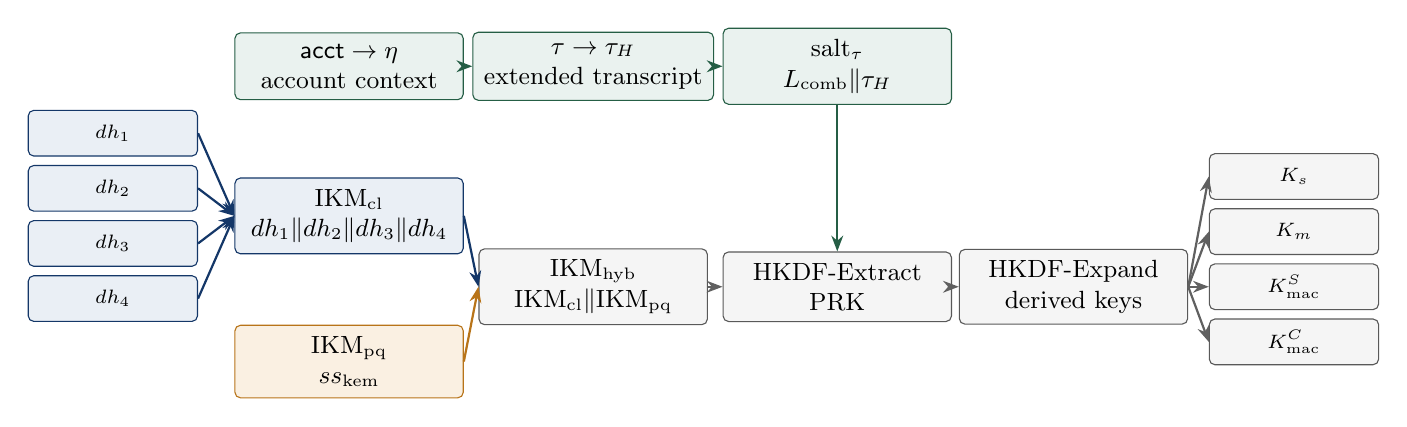
\begin{tikzpicture}[
  font=\small,
  >=Stealth,
  block/.style={draw,rounded corners=2pt,minimum width=2.9cm,
    minimum height=0.72cm,align=center,inner sep=4pt},
  smallblock/.style={draw,rounded corners=2pt,minimum width=2.15cm,
    minimum height=0.58cm,align=center,inner sep=3pt,font=\scriptsize},
  arrow/.style={-{Stealth[length=2mm]},thick},
  cl/.style={fill=eclblue!9,draw=eclblue!75!black},
  pq/.style={fill=eclgold!13,draw=eclgold!85!black},
  ctx/.style={fill=eclgreen!10,draw=eclgreen!75!black},
  kdf/.style={fill=gray!8,draw=gray!70!black}
]
  \node[smallblock,cl] (dh1) at (0,0.9) {$dh_1$};
  \node[smallblock,cl] (dh2) at (0,0.2) {$dh_2$};
  \node[smallblock,cl] (dh3) at (0,-0.5) {$dh_3$};
  \node[smallblock,cl] (dh4) at (0,-1.2) {$dh_4$};
  \node[block,cl] (classical) at (3.0,-0.15)
    {$\mathrm{IKM}_{\mathrm{cl}}$\\$dh_1\|dh_2\|dh_3\|dh_4$};

  \node[block,pq] (kem) at (3.0,-2.0)
    {$\mathrm{IKM}_{\mathrm{pq}}$\\$ss_{\mathrm{kem}}$};
  \node[block,kdf] (combined) at (6.1,-1.05)
    {$\mathrm{IKM}_{\mathrm{hyb}}$\\$\mathrm{IKM}_{\mathrm{cl}}\|
      \mathrm{IKM}_{\mathrm{pq}}$};

  \node[block,ctx] (acct) at (3.0,1.75)
    {$\acct \rightarrow \eta$\\account context};
  \node[block,ctx] (tau) at (6.1,1.75)
    {$\tau \rightarrow \tau_H$\\extended transcript};
  \node[block,ctx] (salt) at (9.2,1.75)
    {$\mathrm{salt}_{\tau}$\\$\Label{comb}\|\tau_H$};

  \node[block,kdf] (extract) at (9.2,-1.05)
    {HKDF-Extract\\$\mathrm{PRK}$};
  \node[block,kdf] (expand) at (12.2,-1.05)
    {HKDF-Expand\\derived keys};
  \node[smallblock,kdf] (ks) at (15.0,0.35) {$K_s$};
  \node[smallblock,kdf] (km) at (15.0,-0.35) {$K_m$};
  \node[smallblock,kdf] (macs) at (15.0,-1.05) {$K_{\mathrm{mac}}^S$};
  \node[smallblock,kdf] (macc) at (15.0,-1.75) {$K_{\mathrm{mac}}^C$};

  \foreach \x in {dh1,dh2,dh3,dh4} {
    \draw[arrow,eclblue!75!black] (\x.east) -- (classical.west);
  }
  \draw[arrow,eclblue!75!black] (classical.east) -- (combined.west);
  \draw[arrow,eclgold!85!black] (kem.east) -- (combined.west);
  \draw[arrow,gray!75!black] (combined.east) -- (extract.west);
  \draw[arrow,eclgreen!75!black] (acct.east) -- (tau.west);
  \draw[arrow,eclgreen!75!black] (tau.east) -- (salt.west);
  \draw[arrow,eclgreen!75!black] (salt.south) -- (extract.north);
  \draw[arrow,gray!75!black] (extract.east) -- (expand.west);
  \foreach \x in {ks,km,macs,macc} {
    \draw[arrow,gray!75!black] (expand.east) -- (\x.west);
  }
\end{tikzpicture}
}
\caption{Transcript-bound hybrid key schedule. Classical 4DH material and
the ML-KEM shared secret are extracted under a transcript-derived salt before
expansion into session, master, and confirmation keys.}
\label{fig:hybrid-key-schedule}
\end{figure}

\textbf{Key derivation.} Let
$\KLabel{s}$, $\KLabel{m}$, $\KLabel{macS}$, and $\KLabel{macC}$
denote fixed labels for the session key, the master key, and the two
confirmation keys:
\begin{align}
  K_s &= \mathrm{HKDF\text{-}Expand}(\mathrm{PRK}, \KLabel{s}, 64),
  \notag\\
  K_m &= \mathrm{HKDF\text{-}Expand}(\mathrm{PRK}, \KLabel{m}, 32),
  \notag\\
  K_{\mathrm{mac}}^S &= \mathrm{HKDF\text{-}Expand}(\mathrm{PRK},
    \KLabel{macS}, 64),
  \notag\\
  K_{\mathrm{mac}}^C &= \mathrm{HKDF\text{-}Expand}(\mathrm{PRK},
    \KLabel{macC}, 64).
  \label{eq:key-derivation}
\end{align}
The resulting second authentication message is
\begin{equation}
  \begin{aligned}
    \mathrm{KE2} &= n_S \| E_S \| \mathrm{CredResp} \| {}\\
    &\quad \mathrm{HMAC}(K_{\mathrm{mac}}^S, \tau) \| ct_{\mathrm{kem}}
      \quad(1376~\text{bytes of payload}).
  \end{aligned}
\end{equation}
In wire format, the message is $v \| \mathrm{KE2}$ and occupies
1377~bytes.

\subsubsection{Generation of KE3 from Initiator to Record-Holding Responder}

\begin{enumerate}
  \item OPRF finalization, opening of the envelope, and recovery of the
        responder public key, initiator static key, and initiator public
        key;
  \item Mirror 4DH:
        $dh_1 = sk_C \cdot PK_S$,
        $dh_2 = e_C \cdot PK_S$, $dh_3 = sk_C \cdot E_S$,
        $dh_4 = e_C \cdot E_S$ (additional binding of the ephemeral
        components at the level of 4DH intuition);
  \item Decapsulation:
        $ss_{\mathrm{kem}} =
        \mathrm{ML\text{-}KEM\text{-}768.Decaps}(sk_{\mathrm{kem}},
        ct_{\mathrm{kem}})$; $sk_{\mathrm{kem}}$ is destroyed
        immediately;
  \item Re-derivation of the same PRK; verification of
        $\mathrm{HMAC}(K_{\mathrm{mac}}^S, \tau)$ by means of a
        constant-time bytewise comparison without early exit;
  \item $\mathrm{KE3} = \mathrm{HMAC}(K_{\mathrm{mac}}^C, \tau)$
        (64~bytes of payload, 65~bytes including the version prefix).
\end{enumerate}

\subsubsection{Completion at the Record-Holding Responder}

KE3 is verified using a constant-time comparison routine. Upon success,
the pair $(K_s, K_m)$ becomes available to both parties, thereby
confirming mutual authentication. Completion is fail closed: if KE3 is
malformed, expired, or fails MAC verification after KE2 has been
generated, no session key is exported; responder-held copies of $K_s$,
$K_m$, $ss_{\mathrm{kem}}$, the expected initiator MAC, and the
responder ephemeral secrets are zeroized; and the state becomes
terminal or invalidated so the same KE2 state cannot be retried as an
authentication oracle.

\subsection{Transcript-Binding Check}

The transcript definition in Eq.~\eqref{eq:hybrid-transcript} is the
normative binding point for the hybrid construction. It requires both
$pk_{\mathrm{kem}}$ and $ct_{\mathrm{kem}}$ to be MAC-authenticated
together with the listed classical authentication fields and the
account-context hash $\eta$. The authentication OPRF blinding value
$B_{\mathrm{auth}}$ is validated and evaluated in the OPRF path rather
than included in $\tau$, and the version byte is handled by the
wire-format parser before transcript construction. Any implementation
that omits the listed post-quantum fields or $\eta$ from $\tau$
implements a different protocol. The resulting transcript binds the
classical and post-quantum key-schedule inputs to a concrete account
under the versioned wire format in which the messages are parsed.

% ============================================================
\section{Security Analysis}
% ============================================================

\subsection{Formal Analysis of Security Properties}

\paragraph{Offline guessing under a fixed trust boundary}
The relevant compromise case is deliberately narrow. The adversary is
allowed to obtain the passive server-side storage $\mathrm{rec}$ and the
observable transcripts, but not $\sigoprf$. Under that condition, the
record does not give an efficient offline verifier for dictionary
candidates except through a break of OPRF obliviousness or envelope
security. If $\sigoprf$ is compromised, the problem changes: the attacker
can evaluate the account-specific OPRF path and the remaining work is a
dictionary search with per-guess cost dominated by Argon2id. The claim is
therefore a statement about a specific operational boundary, not about
all possible server compromise cases.

\begin{sketchproof}
Let $S_0,S_1,S_2$ denote the real database-disclosure experiment, the
experiment with randomized OPRF output, and the experiment with a hidden
envelope plaintext, respectively. Let $\mathcal{Q}_{\mathrm{on}}$ be the
set of password candidates submitted through online protocol attempts.
\textbf{Case 1: \textnormal{$\sigoprf$ not compromised.}}
Without the account-specific OPRF key, the adversary cannot compute
$y_{\mathrm{oprf}}$ via~\eqref{eq:oprf-output}, and hence cannot
reconstruct $x_{\mathrm{ksf}}$, $\mathrm{salt}_{\mathrm{ksf}}$, or
$\mathrm{rwd}$ via~\eqref{eq:rwd}. The envelope record therefore does
not provide an effective offline password-checking oracle. Replacing
the OPRF output with a random value yields
\[
  |\Pr[S_1] - \Pr[S_0]| \leq
  \mathrm{Adv}_{\mathrm{OPRF}}^{\mathrm{obliv}}
  \leq \mathrm{Adv}_{\mathrm{CDH}}^{\mathrm{Ristretto255}}.
\]
\textbf{Envelope-hiding transition.} Next replace the envelope with an
encryption of a random string, reducing the change in success probability
to the authenticated-encryption security of XSalsa20-Poly1305:
\[
  |\Pr[S_2] - \Pr[S_1]| \leq
  \mathrm{Adv}_{\mathrm{XSalsa20\text{-}Poly1305}}^{\mathrm{AE}}.
\]
\textbf{Consequence.} In the absence of compromise of
$\sigoprf$, the best available strategy collapses to online guessing,
whence
\[
  \mathrm{Adv}^{\mathrm{dict}} \leq
  \mathrm{Adv}_{\mathrm{CDH}}^{\mathrm{Ristretto255}} +
  \mathrm{Adv}_{\mathrm{XSalsa20\text{-}Poly1305}}^{\mathrm{AE}} +
  \Pr[\mathrm{pwd} \in \mathcal{Q}_{\mathrm{on}}].
\]
\textbf{Case 2: \textnormal{$\sigoprf$ compromised.}} Then
each dictionary guess $\mathrm{pwd}'$ can be checked offline by
computing $y_{\mathrm{oprf}}'$, then
$x_{\mathrm{ksf}}'$, $\mathrm{salt}_{\mathrm{ksf}}'$, and finally one
attempt to open the envelope. The cost of a single guess is dominated,
both asymptotically and empirically, by Argon2id, that is, by the
procedure~\eqref{eq:rwd}:
\[
  T_{\mathrm{guess}} \approx T_{\mathrm{Argon2id}},\qquad
  C_{\mathrm{offline}} \approx |\mathcal{D}| \cdot T_{\mathrm{guess}}.
\]
For a ranked password distribution and a fixed compute budget $C_{\mathrm{cpu}}$, the
number of tested candidates is bounded by the lower of the compute and
memory bottlenecks:
\[
  G \leq
  \min\!\left(
    \left\lfloor \frac{C_{\mathrm{cpu}}}{T_{\mathrm{guess}}} \right\rfloor,\;
    \left\lfloor \frac{B_{\mathrm{mem}}}{256~\mathrm{MiB}} \right\rfloor
      \cdot
      \left\lfloor \frac{T_{\mathrm{wall}}}{T_{\mathrm{guess}}} \right\rfloor
  \right),
\]
where $B_{\mathrm{mem}}$ is the memory available to parallel guesses and
$T_{\mathrm{wall}}$ is the number of Argon2id time slots in the attack
window. This calculation is intentionally operational rather than
cryptographic: once $\sigoprf$ is lost, protection shifts from the
aPAKE record property to password entropy, KSF cost, rate controls, and
incident response.
\end{sketchproof}

\begin{claim}[Scoped forward secrecy]
Within the compromise model stated above, compromise of the long-term
keys $sk_C$ and $sk_S$ after session completion is argued not to suffice
to recover $K_s$, under the hardness of CDH and the IND-CCA security of
ML-KEM-768.
\end{claim}

\begin{sketchproof}
After compromise of both long-term keys, the terms containing a static
secret can be reconstructed from the public transcript:
$dh_1 = sk_S \cdot PK_C$, $dh_2 = sk_S \cdot E_C$, and
$dh_3 = sk_C \cdot E_S$. The remaining classical term
$dh_4 = e_S \cdot E_C = e_C \cdot E_S$ still requires recovery of a
session ephemeral scalar or a break of CDH on the recorded ephemeral
points. In parallel, $ss_{\mathrm{kem}}$ remains protected under the
IND-CCA security of ML-KEM-768 together with correct erasure and absence
of leakage from the session-local $sk_{\mathrm{kem}}$. Thus
post-session exposure of long-term keys alone does not reconstruct the
full input to the hybrid extractor:
\begin{equation}
  \label{eq:fs-advantage-bound}
  \begin{aligned}
    \mathrm{Adv}^{\mathrm{FS}}
    &\leq
    \min\!\left\{
      \mathrm{Adv}_{\mathrm{CDH}}^{\mathrm{Ristretto255}},
      \mathrm{Adv}_{\mathrm{ML\text{-}KEM}}^{\mathrm{IND\text{-}CCA}}
    \right\}
    + \mathrm{Adv}_{\mathrm{HKDF}}^{\mathrm{ext}}.
  \end{aligned}
\end{equation}
\end{sketchproof}

\begin{claim}[MAC-confirmation argument]
Under the PRF model for HMAC-SHA-512, successful confirmation-token
forgery after $q_{\mathrm{mac}}$ verification attempts is modeled by the
estimate
\[
  \mathrm{Adv}^{\mathrm{mac\text{-}conf}} \leq
  \mathrm{Adv}_{\mathrm{HMAC}}^{\mathrm{PRF}} +
  q_{\mathrm{mac}} / 2^{512}.
\]
\end{claim}

\paragraph{Interpretive claim on the hybrid-source combiner}
Let
\[
  \begin{aligned}
    \mathrm{IKM}_{\mathrm{cl}}
      &= \operatorname{Encode}(dh_1) \| \operatorname{Encode}(dh_2)\\
      &\quad \| \operatorname{Encode}(dh_3) \|
        \operatorname{Encode}(dh_4),\\
    \mathrm{IKM}_{\mathrm{pq}} &= ss_{\mathrm{kem}}.
  \end{aligned}
\]
If, for a fixed transcript $\tau$, at least one of the sources
$\mathrm{IKM}_{\mathrm{cl}}$ or $\mathrm{IKM}_{\mathrm{pq}}$ remains
computationally hidden and retains sufficient entropy for the extractor
model, then the extracted pre-key is
\[
  \mathrm{PRK} =
  \mathrm{HKDF\text{-}Extract}(\mathrm{salt}_{\tau},
    \mathrm{IKM}_{\mathrm{cl}} \| \mathrm{IKM}_{\mathrm{pq}}).
\]
This value is treated as pseudorandom under the standard extractor
interpretation of HKDF-Extract. This gives the intended hybrid-source
reading of the key schedule: explicit recovery of the real session key from the
transcript requires compromise of \emph{both} sources. The statement is not a
standalone computational proof of the combiner. It is an
extractor-based interpretation that is used consistently in the
subsequent symbolic model and implementation checks.

\begin{sketchproof}
Let $S$ denote the source among
$\{\mathrm{IKM}_{\mathrm{cl}}, \mathrm{IKM}_{\mathrm{pq}}\}$ that
remains computationally hidden relative to the fixed transcript $\tau$
and retains sufficient entropy in the extractor model, and let $X$
denote the other source. Then
$\mathrm{IKM}_{\mathrm{cl}} \| \mathrm{IKM}_{\mathrm{pq}}$ may be
written as $S \| X$. The standard extractor property of HMAC-based
HKDF-Extract~\cite{krawczyk2010} suggests that if $S$ is hidden from the
adversary with sufficient entropy, then $\mathrm{PRK}$
remains pseudorandom even for arbitrary $X$. This yields the upper
bound: indistinguishability of the final key can fail only
through a break of the surviving source or a break of the extractor
itself:
\begin{equation}
  \label{eq:hybrid-advantage-bound}
  \begin{aligned}
    \mathrm{Adv}^{\mathrm{hybrid}}
    &\leq
    \min\!\left\{
      \mathrm{Adv}_{\mathrm{CDH}}^{\mathrm{Ristretto255}},
      \mathrm{Adv}_{\mathrm{ML\text{-}KEM}}^{\mathrm{IND\text{-}CCA}}
    \right\}
    + \mathrm{Adv}_{\mathrm{HKDF}}^{\mathrm{ext}}.
  \end{aligned}
\end{equation}
\end{sketchproof}

This bound explains the hybrid-source interpretation used in the sequel. If
at least one of the two sources remains computationally hidden, and
HKDF-Extract behaves as an extractor, then the derived PRK remains
pseudorandom up to the additive extractor term. The interpretation is
narrow: in this reduction sketch and in the symbolic analysis below,
compromise of the final key is modeled as requiring simultaneous
weakening of the classical and post-quantum layers.
Figure~\ref{fig:hybrid-condition-surface} visualizes this interpretation.

\begin{figure}[htbp]
\centering
\resizebox{0.88\textwidth}{!}{%
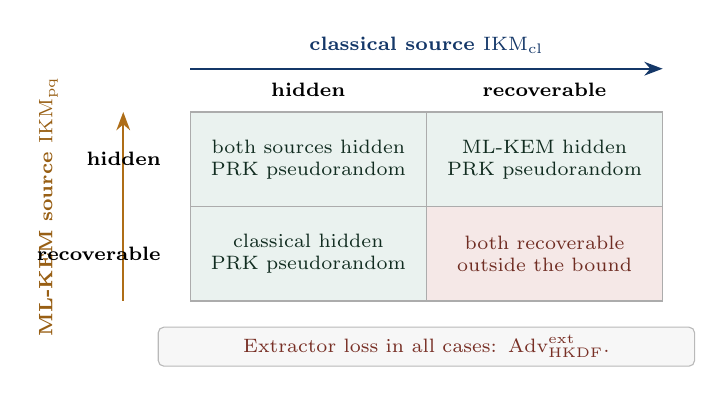
\begin{tikzpicture}[
  font=\scriptsize,
  header/.style={font=\scriptsize\bfseries,align=center},
  note/.style={draw=gray!55,rounded corners=2pt,fill=gray!6,
    align=center,inner sep=3pt,font=\scriptsize},
  >=Stealth
]
  \coordinate (A) at (1.6,0.1);
  \coordinate (B) at (7.6,2.5);

  \fill[eclgreen!10] (1.6,1.3) rectangle (4.6,2.5);
  \fill[eclgreen!10] (4.6,1.3) rectangle (7.6,2.5);
  \fill[eclgreen!10] (1.6,0.1) rectangle (4.6,1.3);
  \fill[eclred!12] (4.6,0.1) rectangle (7.6,1.3);

  \draw[gray!65] (A) rectangle (B);
  \draw[gray!65] (4.6,0.1) -- (4.6,2.5);
  \draw[gray!65] (1.6,1.3) -- (7.6,1.3);

  \node[header,text=eclblue!75!black] at (4.6,3.35)
    {classical source $\mathrm{IKM}_{\mathrm{cl}}$};
  \draw[->,thick,eclblue!75!black] (1.6,3.05) -- (7.6,3.05);

  \node[header,rotate=90,text=eclgold!70!black] at (-0.20,1.30)
    {ML-KEM source $\mathrm{IKM}_{\mathrm{pq}}$};
  \draw[->,thick,eclgold!80!black] (0.75,0.10) -- (0.75,2.50);

  \node[header] at (3.10,2.78) {hidden};
  \node[header] at (6.10,2.78) {recoverable};
  \node[header,anchor=east] at (1.35,1.90) {hidden};
  \node[header,anchor=east] at (1.35,0.70) {recoverable};

  \node[align=center,text=eclgreen!35!black,text width=2.65cm] at (3.10,1.90)
    {both sources hidden\\$\mathrm{PRK}$ pseudorandom};
  \node[align=center,text=eclgreen!35!black,text width=2.65cm] at (6.10,1.90)
    {ML-KEM hidden\\$\mathrm{PRK}$ pseudorandom};
  \node[align=center,text=eclgreen!35!black,text width=2.65cm] at (3.10,0.70)
    {classical hidden\\$\mathrm{PRK}$ pseudorandom};
  \node[align=center,text=eclred!65!black,text width=2.65cm] at (6.10,0.70)
    {both recoverable\\outside the bound};

  \node[note,text=eclred!70!black,text width=6.6cm] at (4.60,-0.48)
    {Extractor loss in all cases:
    $\mathrm{Adv}_{\mathrm{HKDF}}^{\mathrm{ext}}$.};
\end{tikzpicture}
}
\caption{Condition map for the hybrid-combiner interpretation used in
Eq.~\eqref{eq:hybrid-advantage-bound}. Rows and columns describe whether
the classical or ML-KEM source remains hidden relative to a fixed
transcript. Under the extractor interpretation, the PRK remains
pseudorandom whenever at least one source remains hidden; simultaneous
recovery of both sources is the source-level condition not ruled out by
the bound, up to the additive extractor term.}
\label{fig:hybrid-condition-surface}
\end{figure}

\subsection{Resistance to Known Attacks}

\textbf{Offline dictionary attacks.} The protection claim is stated for
\emph{database compromise without compromise of $\sigoprf$}. Under this
condition, three independent layers
operate: (1)~OPRF, because without the responder-side OPRF key
$k_{\mathrm{oprf}}$ the adversary cannot compute $\mathrm{rwd}$;
(2)~Argon2id with MODERATE parameters (256~MiB, 3 iterations), for
which one guess costs approximately
$T_{\mathrm{guess}} \approx 0.84$~s on the benchmarking platform, so a
sequential exhaustive dictionary search scales as
$C_{\mathrm{offline}} \approx |\mathcal{D}| \cdot T_{\mathrm{guess}}$;
and (3)~XSalsa20-Poly1305, because verification of a candidate requires
successful authenticated decryption. If $\sigoprf$ is
compromised, this claim does not automatically transfer to the new
threat model and requires separate analysis.

\textbf{Man-in-the-middle attack.} The transcript $\tau$ contains the
listed public protocol elements, including $pk_{\mathrm{kem}}$ and
$ct_{\mathrm{kem}}$. Modification of any transcript-bound field results
in MAC mismatch; other malformed fields fail during parsing, OPRF or
envelope processing, or key confirmation.

\textbf{Replay attack.} Ephemeral nonces (192 bits) and ephemeral keys
are generated afresh for every session. For $N$ sessions using uniformly
sampled 192-bit nonces, the birthday-bound collision probability is
approximately $N(N-1)/2^{193}$.

\textbf{Harvest-now-decrypt-later attack.} If the classical
$dh_1,\ldots,dh_4$ terms are later recovered by a quantum adversary, the
hybrid key still depends on $ss_{\mathrm{kem}}$, whose protection is tied
to ML-KEM-768 and the Module-LWE assumption.

\textbf{Long-term responder-key exposure.} Compromise of $sk_S$ permits
impersonation of the record-holding responder in future sessions and makes the
static-responder DH terms computable from a recorded transcript, including
$dh_1$ and $dh_2$. The narrower post-session claim is that $sk_S$ alone
does not reconstruct a completed hybrid session: it does not reveal the
initiator static secret, the responder ephemeral scalar, the
ephemeral--ephemeral term $dh_4$, or the ML-KEM shared secret
$ss_{\mathrm{kem}}$, which depends on the destroyed
$sk_{\mathrm{kem}}$. The protection statement is therefore scoped to
recovery of the recorded hybrid session key, not to impersonation after
the responder key has been lost.

\textbf{Timing and microarchitectural side channels.} MAC comparisons
are performed by constant-time bytewise comparison without early exit,
and secrets are zeroized on both successful and rejected paths. The
implementation relies on constant-time-oriented Ristretto255 and ML-KEM
components, but the evidence here does not include cache-trace,
branch-prediction, power, fault-injection, or compiler-level leakage
analysis. Side-channel resistance should therefore be treated as an
engineering requirement for a hardened deployment, not as a theorem
established by the symbolic models.

\subsection{Formal Verification}

\subsubsection{Verification Overview}

The protocol was analyzed with two symbolic tools in the Dolev--Yao
model: ProVerif~2.05 and Tamarin~Prover~1.10.0. The purpose of this
analysis is to check the structure of the protocol argument, not to
certify the reference implementation line by line. ProVerif is used in
separate secrecy and authentication models, whereas Tamarin is applied
to a verified surrogate 4DH model. The results are therefore read
together with the modeling boundaries and with the executable artifact
that exercises serialization, state handling, and external-call behavior
\cite{cremers2012,basin2018}.

\begin{table}[htbp]
\caption{Symbolic verification summary and modeling boundary}
\label{tab:verification-summary}
\centering\scriptsize
\begin{tabularx}{\textwidth}{@{}L{3.4cm}L{2.4cm}L{3.3cm}X@{}}
\toprule
Property & ProVerif & Tamarin & Boundary \\
\midrule
Session-key secrecy & confirmed & confirmed in 27 steps & Symbolic secrecy only; no side-channel or compiled-code claim. \\
Password secrecy on the wire & confirmed & confirmed in 3 steps & Password absence is checked in the model trace abstraction. \\
Classical forward secrecy & not modeled & confirmed in 119 steps & Uses the surrogate 4DH representation. \\
Post-quantum contribution & not modeled separately & represented through the hybrid-source lemma & Does not constitute an IND-CCA proof of ML-KEM. \\
Initiator authentication & confirmed & confirmed in 32 steps & Correspondence assertion under the modeled event structure. \\
Responder authentication & confirmed & confirmed in 17 steps & Correspondence assertion under the modeled event structure. \\
Injective mutual authentication & confirmed & follows from authentication lemmas & Not a proof about API misuse or error formatting. \\
Hybrid-source interpretation & not modeled & supported in 29 steps & Evidence for the stated abstraction, not a computational combiner theorem. \\
Offline guessing in the DB model & not modeled & supported in 4 steps & Assumes $\sigoprf$ remains outside the compromised store. \\
Executability & not applicable & confirmed in 16 steps & Confirms existence of an honest completion trace. \\
\midrule
Total & 5/5 queries & 8/8 lemmas & Results belong to separate symbolic abstractions. \\
\bottomrule
\end{tabularx}
\end{table}

\begin{table}[htbp]
\caption{Executable artifact checks and what they do not prove}
\label{tab:executable-checks}
\centering\scriptsize
\begin{tabularx}{\textwidth}{@{}L{3.4cm}L{5.1cm}X@{}}
\toprule
Test area & Representative checks & Does not prove \\
\midrule
Wire format and versioning & Exact KE1/KE2/KE3 lengths, unsupported-version rejection, malformed-length rejection & Correctness of every future serialization profile. \\
Transcript binding & Mutation of transcript-bound fields, including post-quantum material and account context & A general composition theorem for all hybrid PAKEs. \\
State lifecycle & State consumption, replay rejection, failure-state invalidation, zeroization boundaries & Absence of all memory-forensics or side-channel leakage. \\
External adapter contract & Public error categories, buffer ownership, safe release paths & Correct integration by arbitrary foreign callers. \\
Benchmark harnesses & Primitive and protocol workloads under Criterion & Universal timing behavior across platforms. \\
\midrule
Total test outcome & 157 passed, 1 intentionally ignored slow regression & Machine-checked implementation correctness. \\
\bottomrule
\end{tabularx}
\end{table}

Tables~\ref{tab:verification-summary} and~\ref{tab:executable-checks}
separate evidence that is often conflated. ProVerif is most useful for
message logic and correspondence properties in a simplified
unbounded-session setting; Tamarin records stateful properties under the
surrogate 4DH abstraction; and the executable test suite checks concrete
state-machine behavior that symbolic tools intentionally abstract away:
wire-format parsing, version and length rejection, transcript-field
mutation, replay rejection, failure-state consumption, zeroization
boundaries, and external-adapter error contracts. These tests do not
replace symbolic analysis; they bind the formalized protocol structure
to implementation behavior that callers actually exercise.

\subsubsection{ProVerif 2.05}

Toolchain: ProVerif~2.05 with OCaml~5.4.0. Two
complementary models were used: a baseline secrecy model and a separate
authentication model, both archived in the accompanying artifact
package. The split into two models is deliberate: a single saturated
model did not yield stable convergence for all queries simultaneously.
The ProVerif results provide two compatible but distinct views of the
same protocol.

\begin{table}[htbp]
\caption{Split ProVerif models and their abstractions}
\label{tab:proverif-split}
\centering\scriptsize
\begin{tabularx}{\textwidth}{@{}L{3.0cm}L{4.6cm}X@{}}
\toprule
Model & Queries checked & Principal abstraction \\
\midrule
Secrecy model & Session-key secrecy and password secrecy on the
wire & Authentication events are simplified so that secrecy saturation
converges reliably across unbounded sessions. \\
Authentication model & Initiator, responder, and injective mutual
correspondence & Key-material secrecy is abstracted to focus the model
on event ordering and agreement. \\
\bottomrule
\end{tabularx}
\end{table}

The split is acceptable only because both models use the same message
roles, transcript fields, compromise events, and success/failure events.
It would be misleading to add their outcomes as though they were a
single monolithic proof; they are two consistency checks over the same
protocol description.

The most informative query for mutual authentication is P5c (injective
mutual correspondence): it states that each successful completion on
the responder side corresponds to a distinct matching completion on the
initiator side for the same pair of parties and the same session key. A
positive result means that successful completion on the responder side
cannot be explained by replaying a single successful trace across
multiple initiator completions. This result is not a computational proof
of the implementation: the model omits side channels, variation in
error formatting, timing-related leakage, and a range of network-level
details that remain the domain of implementation testing.

\subsubsection{Tamarin Prover 1.10.0}

Toolchain: Tamarin~1.10.0 (Maude~3.4). A surrogate model of the hybrid
combiner was verified; the archived 4DH proof log records a total
solving time of \textbf{53.84~seconds} for all eight lemmas.
Table~\ref{tab:tamarin-lemmas} lists the verified lemmas and their
main security interpretation.

\begin{table}[htbp]
\caption{Tamarin lemmas established for the surrogate 4DH model}
\label{tab:tamarin-lemmas}
\centering\small
\begin{tabularx}{\textwidth}{@{}L{4.5cm}rX@{}}
\toprule
Lemma & Steps & Key property \\
\midrule
Session-key secrecy (P1) & 27 & Without corruption events, the adversary cannot derive the session key \\
Password secrecy (P2) & 3 & The password never appears in externally observable model events \\
Forward secrecy (P3) & 119 & The session key remains non-derivable after post-session long-term key compromise, assuming session ephemerals are not disclosed \\
Initiator authenticity (P5a) & 32 & Successful initiator completion requires prior responder participation \\
Responder authenticity (P5b) & 17 & Successful responder completion requires a valid KE3 \\
Hybrid-source interpretation (P6) & 29 & Without compromise of the ephemeral secrets, the 4DH and KEM components are not recovered jointly \\
Offline-guessing resistance in the DB model (P7) & 4 & Database compromise reveals the record but not the OPRF key \\
Executability (correctness) & 16 & A successful protocol-completion trace exists \\
\bottomrule
\end{tabularx}
\end{table}

The verified Tamarin model does not use an embedded Diffie--Hellman
equational theory for the full 4DH construction. Instead, it replaces
4DH with an abstract secret
$\xi_{\mathrm{4dh}} = h(\langle \mathrm{sk}_C,\mathrm{sk}_S,e_C,e_S\rangle)$
and checks which compromise events are required for the adversary to
derive the session key. This abstraction makes automated reasoning
feasible and is interpreted as surrogate symbolic evidence rather than
a formal proof of every concrete Ristretto255 operation. In particular,
the model does not test algebraic independence among $dh_1,\ldots,dh_4$,
canonical point validation, cofactor-related issues, or equality
relationships induced by the group law. Those properties are addressed
by primitive choice, implementation checks, and the reduction sketches,
not by the Tamarin lemma itself.

Lemma P6 is central to the combiner interpretation. It states that from
the establishment of the session key and the absence of disclosure of
the initiator's and responder's ephemeral secrets, non-derivability of
that key for the adversary follows. The machine verification of this
lemma completes positively in 29 steps.

The lemma permits compromise of long-term keys but disallows disclosure
of ephemeral ones. Even with knowledge of the parties' long-term
secrets, the adversary cannot recover the modeled hybrid key material
without access to the ephemeral components represented in the classical
and post-quantum layers. Within this surrogate model, the result
supports the stated hybrid-source interpretation. It does not establish
the same claim for a full equational model of Ristretto255 or replace a
separate formalization of post-quantum forward secrecy.

\subsubsection{Limits of Interpretation}

To avoid overstating the formal results, four principal limitations are
recorded.
\begin{enumerate}
  \item \textbf{Surrogate representation of 4DH.} The verified Tamarin
        model abstracts the 4DH component into a single knowledge
        function. This facilitates the proof but does not replace
        analysis of the concrete algebraic properties of group
        operations, canonical point decoding, or independence of the
        four Diffie--Hellman terms.
  \item \textbf{Split ProVerif models.} Secrecy and authentication are
        studied not in one universal model but in two separate
        artifacts. Hence the 5/5 outcome should be interpreted as the
        aggregate of two mutually consistent models rather than as a
        monolithic proof.
  \item \textbf{Boundary of offline-resistance claims.} Lemma P7 and the
        corresponding executable tests cover database compromise \emph{without}
        compromise of $\sigoprf$. If $\sigoprf$ is exposed, the
        offline-resistance property requires separate analysis and
        should not be transferred automatically from the model.
  \item \textbf{Gap between model and implementation.} Symbolic
        verification does not cover side channels, compiler behavior,
        memory-allocation properties, external-API mistakes, or
        vulnerabilities in external crates. For this reason, the formal
        results reported here complement tests and benchmarks rather than
        substituting for them.
\end{enumerate}

% ============================================================
\section{Implementation and Experimental Evaluation}
% ============================================================

\subsection{Architecture of the Reference Implementation}

The protocol is implemented in \textbf{Rust~1.93.1} as a multi-crate
workspace. Rust was selected for compile-time memory safety, the
ability to keep the cryptographic core free of \codeid{unsafe} blocks,
and the availability of mature secret-zeroization mechanisms.
Table~\ref{tab:code-metrics} summarizes the implementation surface used
for the evaluation.

\begin{table}[htbp]
\caption{Source-code metrics of the workspace}
\label{tab:code-metrics}
\centering\small
\begin{tabular*}{\textwidth}{@{\extracolsep{\fill}}L{3.2cm}L{3.8cm}rL{3.0cm}@{}}
\toprule
Component & Role & LoC & Principal dependencies \\
\midrule
\textbf{Cryptographic core} & Primitives, key derivation, and protocol serialization & 1513 & Ristretto255, ML-KEM, Argon2id \\
\textbf{Initiator pipeline} & Initiator protocol phases & 900 & cryptographic core \\
\textbf{Responder pipeline} & Record-holding responder phases and session completion & 907 & cryptographic core \\
\textbf{Interlanguage layer} & Foreign-call adapter and protocol invocation & 2026 & initiator and responder pipelines \\
\midrule
\textbf{Total (main code)} & & \textbf{5346} & \\
Tests & & 4116 & property-based and regression scenarios \\
Benchmarks & & 1460 & Criterion \\
Formal models & & 1806 & Tamarin, ProVerif \\
\bottomrule
\end{tabular*}
\end{table}

\subsection{Specification-to-Implementation Traceability}

The implementation is organized so that the main protocol statements in
the paper can be checked against concrete artifacts rather than against
informal intent. This traceability is not a proof of correctness, but it
reduces the risk that the specification, implementation, benchmarks, and
adapter documentation drift into describing different protocols.
Table~\ref{tab:traceability} summarizes the correspondence used in the
artifact.

\begin{table}[htbp]
\caption{Traceability between the paper specification and executable artifact}
\label{tab:traceability}
\centering\scriptsize
\begin{tabularx}{\textwidth}{@{}L{3.0cm}L{4.8cm}X@{}}
\toprule
Specification element & Implementation locus & Artifact check \\
\midrule
Wire-format lengths and version prefix & Core type constants and
protocol serialization/parsing routines & Unit tests reject short,
long, and unsupported-version messages; public length accessors expose the
same 1273/1377/65-byte authentication sizes. \\
Account-bound OPRF derivation & OPRF and registration/envelope modules
shared by the initiator and responder crates & OPRF, envelope, and registration
tests cover account-specific derivation, validation failures, and
rejection of malformed public inputs. \\
Hybrid 4DH~+~ML-KEM key path & Initiator authentication, responder
authentication, and ML-KEM helper module & Integration and
property-oriented tests exercise successful completion, tampered KE2/KE3
rejection, replay rejection, and independent session-key agreement. \\
Transcript binding of PQ material and $\acct$ & Authentication-state
construction on both endpoints & Negative tests mutate transcript-bound
fields and require authentication failure rather than silent divergence. \\
State lifetime and zeroization boundary & Initiator state, responder state, and
foreign-call lifecycle wrappers & Regression tests check state consumption,
rejection after invalid transitions, and safe release paths across the
foreign-call boundary. \\
Public external error contract & Initiator and responder adapter modules plus the public
adapter documentation & Adapter lifecycle tests verify that unsupported protocol
versions remain distinguishable at the foreign-call boundary instead of being
collapsed into generic authentication failure. \\
\bottomrule
\end{tabularx}
\end{table}

The important point is methodological. The symbolic models describe the
message structure and compromise assumptions; the executable tests check
whether the executable state machine follows the same message sizes,
labels, version handling, and rejection behavior; and the adapter
documentation exposes the subset of those contracts that external
callers must obey. This separation makes the artifact more directly
auditable because cryptographic claims, implementation invariants, and
foreign-call obligations are
related but not treated as interchangeable evidence.

\subsection{Memory Safety and Secret Zeroization}

For a cryptographic system, security depends not only on the selected
primitives but also on the discipline with which secrets are handled in
process memory. In the implementation studied here, the
cryptographic core and both protocol pipelines are compiled under a
strict no-\codeid{unsafe}-code policy, whereas operations that require
low-level pointer manipulation are confined to a narrow foreign-call boundary.
Such architectural separation does not replace formal analysis of the
implementation, but it limits the defect surface at the
memory-management boundary: use-after-free defects, double release,
loss of correct buffer ownership, and violations of buffer-length
invariants.

Control over secret lifetime is equally important. The
implementation systematically applies automatic zeroization when
objects leave scope together with dedicated wrappers for transient
values, so that sensitive intermediate quantities remain in memory only
for the minimal interval required. This does not eliminate every
possible leak, but it reduces the post-compromise residue of
sensitive data in memory dumps, crash logs, and reused buffers. In particular, the
following values are zeroized:
\begin{itemize}
  \item the user password and the OPRF blinding scalar after OPRF
        finalization;
  \item the ephemeral ML-KEM secret after decapsulation;
  \item the classical 4DH material, the transcript hash, and the PRK
        after derivation of descendant keys;
  \item the account-and-version context hash $\eta$ after completion of
        KE2/KE3;
  \item the initiator and responder state structures upon interruption
        or any rejected completion path.
\end{itemize}

\subsection{Testing and Reproducibility}

The evaluated revision of the workspace contains 157 passing tests and
1 deliberately ignored slow regression scenario. The package includes
unit, integration, property-based, and regression tests for the
protocol lifecycle, wire format, external API contract, OPRF/KEM correctness,
and secure rejection of invalid states.

For archival review, the source snapshot should record the exact commit
identifier and the commands used to reproduce each evidence layer:
\texttt{cargo test --workspace} for executable tests, the documented
Criterion benchmark targets for timing, \texttt{proverif} for the two
ProVerif files, and \texttt{tamarin-prover} for the archived Tamarin
model. The expected review outcome for the snapshot described here is
157 passed tests, one intentionally ignored slow regression, 5/5
ProVerif queries, and 8/8 Tamarin lemmas.

These checks complement the symbolic analysis rather than duplicate it.
Executable tests exercise serialization, version handling, state-lifecycle
invariants, and input-boundary conditions in the executable
implementation; Criterion~0.5.1 benchmarks~\cite{heyer2023} quantify
the cost of the main primitives and protocol phases; archived ProVerif
and Tamarin models document the formal abstractions used for the
security claims.

Benchmarking was performed on a Linux server with two
Intel~Xeon~E5-2650~v4 processors (24 physical cores, 48 hardware
threads, 60~MiB aggregate L3 cache, Ubuntu kernel~6.8.0-111,
Rust~1.93.1) in deterministic optimized-build mode.
Criterion applies bootstrap estimation of the mean and the 95\%
confidence interval; the values reported below should be interpreted
as reproducible estimates for this platform rather than as universal
constants for every environment. Reproducing the full test suite, the
benchmark suite, and the formal models gives an independent check on the
main quantitative and structural claims reported here.

\subsection{Benchmarks of Cryptographic Primitives}

Figure~\ref{fig:runtime-profile} summarizes the scale separation before
the detailed benchmark tables.

\begin{figure}[htbp]
\centering
\resizebox{\textwidth}{!}{%
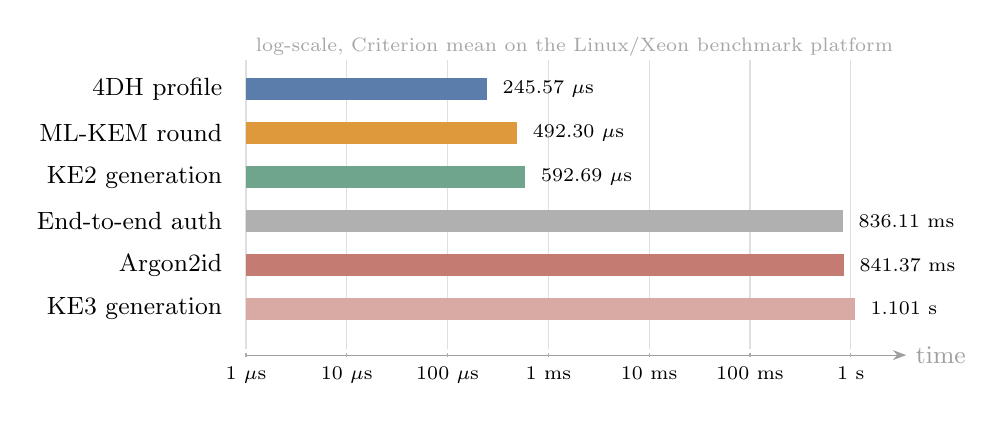
\begin{tikzpicture}[x=1.28cm,y=0.62cm,font=\small,>=Stealth]
  \draw[->,gray!75] (0,0) -- (6.55,0) node[right] {time};
  \foreach \x/\lab in {
    0/{1~$\mu$s},
    1/{10~$\mu$s},
    2/{100~$\mu$s},
    3/{1~ms},
    4/{10~ms},
    5/{100~ms},
    6/{1~s}
  } {
    \draw[gray!25] (\x,0.12) -- (\x,6.05);
    \draw[gray!65] (\x,0.04) -- (\x,-0.04);
    \node[below,font=\scriptsize] at (\x,-0.05) {\lab};
  }

  \node[anchor=east] at (-0.14,5.45) {4DH profile};
  \fill[eclblue!72] (0,5.22) rectangle (2.39,5.68);
  \node[anchor=west,font=\scriptsize] at (2.45,5.45) {245.57~$\mu$s};

  \node[anchor=east] at (-0.14,4.55) {ML-KEM round};
  \fill[eclgold!86] (0,4.32) rectangle (2.69,4.78);
  \node[anchor=west,font=\scriptsize] at (2.75,4.55) {492.30~$\mu$s};

  \node[anchor=east] at (-0.14,3.65) {KE2 generation};
  \fill[eclgreen!70] (0,3.42) rectangle (2.77,3.88);
  \node[anchor=west,font=\scriptsize] at (2.83,3.65) {592.69~$\mu$s};

  \node[anchor=east] at (-0.14,2.75) {End-to-end auth};
  \fill[gray!62] (0,2.52) rectangle (5.92,2.98);
  \node[anchor=west,font=\scriptsize] at (5.98,2.75) {836.11~ms};

  \node[anchor=east] at (-0.14,1.85) {Argon2id};
  \fill[eclred!70] (0,1.62) rectangle (5.93,2.08);
  \node[anchor=west,font=\scriptsize] at (5.99,1.85) {841.37~ms};

  \node[anchor=east] at (-0.14,0.95) {KE3 generation};
  \fill[eclred!45] (0,0.72) rectangle (6.04,1.18);
  \node[anchor=west,font=\scriptsize] at (6.10,0.95) {1.101~s};

  \node[anchor=west,font=\scriptsize,gray!70] at (0,6.32)
    {log-scale, Criterion mean on the Linux/Xeon benchmark platform};
\end{tikzpicture}
}
\caption{Runtime profile on the Linux/Xeon benchmark platform. The
password-hardening step dominates end-to-end latency, while the
post-quantum and classical key-exchange components remain sub-millisecond.}
\label{fig:runtime-profile}
\end{figure}

Table~\ref{tab:micro-bench} gives the primitive-level measurements
behind this profile.

\begin{table}[htbp]
\caption{Benchmark results for cryptographic primitives}
\label{tab:micro-bench}
\centering\small
\begin{tabular*}{\textwidth}{@{\extracolsep{\fill}}llrr@{}}
\toprule
Primitive & Operation & $\hat{\mu}$ & 95\% CI \\
\midrule
Ristretto255 & Key-pair generation & 41.85~$\mu$s & [39.47; 44.28] \\
Ristretto255 & Single DH & 75.93~$\mu$s & [74.11; 77.90] \\
Ristretto255 & 3DH (baseline) & 262.54~$\mu$s & [258.50; 266.58] \\
Ristretto255 & \textbf{4DH (protocol profile)} & \textbf{245.57~$\mu$s} & [242.98; 249.55] \\
ML-KEM-768 & Key-pair generation & 151.48~$\mu$s & [147.39; 155.63] \\
ML-KEM-768 & Encapsulation & 146.50~$\mu$s & [142.58; 150.51] \\
ML-KEM-768 & Decapsulation & 172.74~$\mu$s & [168.74; 176.75] \\
ML-KEM-768 & \textbf{Full round} & \textbf{492.30~$\mu$s} & [479.59; 505.34] \\
OPRF & Blinding & 115.63~$\mu$s & [113.63; 117.64] \\
OPRF & Responder evaluation & 76.39~$\mu$s & [74.95; 77.85] \\
OPRF & Finalization & 109.11~$\mu$s & [107.29; 110.91] \\
HKDF & Extract & 3.63~$\mu$s & [3.52; 3.74] \\
HKDF & Expand (64~bytes) & 2.26~$\mu$s & [2.20; 2.33] \\
HMAC-SHA-512 & 256~bytes & 2.92~$\mu$s & [2.90; 2.94] \\
XSalsa20-Poly1305 & Encrypt 96~bytes & 2.52~$\mu$s & [2.49; 2.57] \\
XSalsa20-Poly1305 & Decrypt 96~bytes & 2.67~$\mu$s & [2.66; 2.69] \\
Argon2id & \textbf{MODERATE} & \textbf{841.37~ms} & [830.54; 851.96] \\
Hybrid combiner & HKDF-Extract (160~bytes) & 2.49~$\mu$s & [2.47; 2.50] \\
\bottomrule
\end{tabular*}
\end{table}

The micro-benchmarks show three stable relationships. First, the full
ML-KEM-768 round ($492.30~\mu$s) and the measured 4DH protocol profile
($245.57~\mu$s) remain sub-millisecond operations, so the
post-quantum layer does not alter the computational class of the
protocol. Second, Argon2id ($841.37$~ms in isolated measurement)
dominates all other components and determines the perceived
authentication latency. Third, the hybrid key-extraction procedure
($2.49~\mu$s) is negligible relative to the KSF and does not
constitute a separate bottleneck.

\subsection{Protocol-Level Benchmarks}

The phase measurements and the complete authentication measurement are
separate Criterion workloads with different state-initialization and
batching boundaries. They are therefore not additive. Table~\ref{tab:protocol-bench}
reports scenario-level timings rather than a decomposition whose rows
sum to the end-to-end value.

\begin{table}[htbp]
\caption{Benchmark results for protocol-level scenarios; rows are separate
Criterion workloads and are not additive}
\label{tab:protocol-bench}
\centering\scriptsize
\begin{tabularx}{\textwidth}{@{}L{2cm}L{3.8cm}rrX@{}}
\toprule
Phase & Measurement scenario & $\hat{\mu}$ & 95\% CI & Main cost \\
\midrule
Registration & Registration-request creation & 127.37~$\mu$s & [125.24; 130.09] & OPRF blinding \\
Registration & Responder response creation & 71.42~$\mu$s & [70.98; 71.84] & OPRF evaluation \\
Registration & Registration completion & \textbf{1.065~s} & [993.93~ms; 1.143~s] & \textbf{Argon2id} \\
Authentication & KE1 generation & 304.87~$\mu$s & [288.05; 322.18] & OPRF + ML-KEM keygen \\
Authentication & KE2 generation & 592.69~$\mu$s & [582.16; 606.72] & 4DH + ML-KEM encaps. \\
Authentication & KE3 generation at the initiator & \textbf{1.101~s} & [1.034; 1.169]~s & \textbf{Argon2id} + decapsulation \\
Authentication & Final responder verification & 2.61~$\mu$s & [2.31; 3.06] & MAC verification \\
\midrule
Full & End-to-end authentication cycle & \textbf{836.11~ms} & [825.41; 847.99] & \textbf{Argon2id} \\
\bottomrule
\end{tabularx}
\end{table}

Responder KE2 generation remains a sub-millisecond operation, whereas Argon2id
contributes the overwhelming share of time.

\subsection{Key Quantitative Findings and Implementation Implications}

The isolated responder profile shows that the responder's cryptographic
core remains compatible with high-throughput deployment:
isolated KE2 generation takes 592.69~$\mu$s, whereas final responder
verification takes only 2.61~$\mu$s. This yields a theoretical upper
bound of approximately $1.69 \times 10^3$ authentications per second
per core for a cryptography-bound responder, excluding database access,
telemetry, and business logic.

For the complete AKE without the KSF, the post-quantum component adds
379.45~$\mu$s ($+48.3\%$) of CPU time; against the Argon2id background,
however, this excess shrinks to approximately $0.045\%$ of a typical
end-to-end scenario. The principal trade-off is not CPU cost but
network volume: the complete handshake occupies
2715~bytes in wire format, that is, 2272~bytes more than the classical
variant at the same three-message interaction profile.

\paragraph{Comparative claim relative to classical OPAQUE}
Let $M_{\mathrm{opq}}, R_{\mathrm{opq}}, C_{\mathrm{opq}}, W_{\mathrm{opq}}$
denote, respectively, the message count, network round-trip cost,
cryptographic computation, and communication volume of canonical
3DH-OPAQUE without the KSF, and let
$M_{\mathrm{hyb}}, R_{\mathrm{hyb}}, C_{\mathrm{hyb}}, W_{\mathrm{hyb}}$
denote the corresponding quantities for Hybrid PQ-OPAQUE. Let
$C_{\mathrm{misc}}$ collect the fixed transcript-binding, serialization,
and key-derivation work introduced by the hybrid path. Then
\[
  \begin{aligned}
    M_{\mathrm{hyb}} &= M_{\mathrm{opq}} = 3,\\
    R_{\mathrm{hyb}} &= R_{\mathrm{opq}} = \tfrac{3}{2}\,\mathrm{RTT},\\
    C_{\mathrm{hyb}} &= C_{\mathrm{opq}} + C_{\mathrm{DH}} +
      C_{\mathrm{KEM}} + C_{\mathrm{misc}},\\
    W_{\mathrm{hyb}} &= W_{\mathrm{opq}} + \Delta W,\qquad
      \Delta W = 2272~\text{bytes}.
  \end{aligned}
\]
On the benchmark platform, this corresponds to a measured increase of
$C_{\mathrm{DH}} + C_{\mathrm{KEM}} + C_{\mathrm{misc}}
\approx 379.45~\mu$s without the
KSF. Compared with the established baseline of classical OPAQUE, the
cost for honest parties rises additively, and the interaction profile is
unchanged. Within the present threat model, explicit compromise of the
final key material is not reducible to weakening the classical
contribution alone; it is interpreted as requiring compromise of both the
classical and post-quantum layers.
Table~\ref{tab:baseline-comparison} states the same comparison in
structural form.

\begin{table}[htbp]
\caption{Comparison of Hybrid PQ-OPAQUE with canonical 3DH-OPAQUE}
\label{tab:baseline-comparison}
\centering\scriptsize
\begin{tabularx}{\textwidth}{@{}L{3.3cm}L{2.9cm}L{3.1cm}X@{}}
\toprule
Aspect & 3DH-OPAQUE & Hybrid PQ-OPAQUE & Interpretation \\
\midrule
Interaction profile & 3 messages, 1.5 RTTs & 3 messages, 1.5 RTTs & Protocol interaction is unchanged \\
Computational complexity for honest parties & Baseline 3DH path & $+1$ additional DH, $+$ KEM, $+$ fixed transcript/KDF work & The increase is additive rather than structural \\
Communication complexity & Baseline handshake volume & $+2272$ bytes in wire format & The principal practical trade-off shifts to transport \\
Key-compromise condition & Weakening of the classical contribution & Compromise of both the classical and PQ layers & The recovery condition is stricter within the present threat model \\
\bottomrule
\end{tabularx}
\end{table}

% ============================================================
\section{Discussion of Results}
% ============================================================

\subsection{Interpretation of the Formal and Experimental Evidence}

The evidence should be read as layered rather than monolithic. ProVerif
addresses secrecy and correspondence in symbolic models, Tamarin records
stateful properties of the surrogate 4DH construction, and the Rust test
suite checks executable behavior that symbolic tools do not model:
serialization, state lifetime, boundary checks, version handling, and the
external API contract. These layers point to the same protocol description, but
they do not have the same evidentiary status.

The least automatic part of the argument is the hybrid-source reading of the
combiner. It is supported by the extractor rationale and by the
surrogate Tamarin lemma, but it is still weaker than a full
computational proof. This distinction is important because the paper is
not claiming that the implementation is machine-verified; it claims that
the design, models, tests, and measurements are mutually consistent
under the stated assumptions.
Table~\ref{tab:claim-scope} separates these claims from their
boundaries.

\begin{table}[htbp]
\caption{Scope of the main claims and supporting evidence}
\label{tab:claim-scope}
\centering\scriptsize
\begin{tabularx}{\textwidth}{@{}L{3.0cm}L{5.2cm}X@{}}
\toprule
Claim & Evidence used in the paper & Boundary of the claim \\
\midrule
Fixed-round hybridization & Explicit message syntax, transcript
definitions, wire-format accounting, and Rust serialization tests &
The construction is OPAQUE-like and does not claim complete
RFC~9807 conformance. \\
Transcript-bound post-quantum contribution & Key-schedule equations,
context binding through $\acct$, formal models, and integration tests &
The formal tools reason about symbolic abstractions, not the compiled
binary or side-channel behavior. \\
Resistance to database-only offline guessing & OPRF-key separation,
database-compromise model, negative regression tests, and the stated
trust boundary for $\sigoprf$ & The claim does not survive compromise of
the OPRF root secret or a deployment that stores it with the password
database. \\
Hybrid-source key dependence & HKDF extractor rationale, the
surrogate 4DH Tamarin lemma, and agreement between the specification and
implementation paths & This is evidence for the intended combiner
interpretation, not a full computational proof of the hybrid PAKE. \\
Practical overhead is dominated by the KSF & Criterion measurements for
primitive costs, end-to-end authentication, and message-size accounting &
The absolute timings are platform-specific and must be recalibrated for
mobile, embedded, or high-latency deployments. \\
\bottomrule
\end{tabularx}
\end{table}

\subsection{Performance, KSF Parameters, and the Trust Boundary}

The performance profile is governed mainly by Argon2id; ML-KEM-768 and
4DH remain sub-millisecond components. The relevant deployment constraint
is therefore not the absolute cost of ML-KEM-768, but the choice of KSF
profile for the target initiator population. The selected profile is
appropriate for web and B2B settings, whereas mobile and edge
deployments may require separate KSF calibration and stricter rate
limiting.

The trust boundary around $\sigoprf$ is not a cosmetic detail. Resistance
to offline guessing is claimed only for database compromise
\emph{without} compromise of that secret. In operational terms,
$\sigoprf$ functions as the root cryptographic secret of the service and
requires separated storage, segregated access, minimal memory residency,
and a rotation policy that treats OPRF-key derivation as privileged
cryptographic state.

A practical advantage of the migration path is that the
post-quantum component remains ephemeral and does not enlarge the
registration record. Migration is concentrated in the application-layer
authentication logic, version negotiation, and contextual binding of
$\acct$. The growth of the wire format to 2715~bytes, however, makes
transport constraints more consequential than in classical OPAQUE: for
TCP/QUIC this is largely a buffering issue, whereas datagram
deployments also face fragmentation and MTU concerns.

\subsection{Migration, Compatibility, and Operational Viability}

The construction can be deployed without redesign of the entire
identity stack for two reasons. First, the registration record does not
accumulate long-lived post-quantum material, because ML-KEM appears
only in the ephemeral authentication path. Second, explicit wire-format
versioning and contextual binding of $\acct$ permit staged rollout
without invalidating existing user state. For operators, migration is
therefore closer to controlled protocol evolution than to complete
credential re-issuance.

Operational compatibility also matters.
Authentication interacts with login-attempt limits, logging, account
recovery, anti-fraud analysis, and audit requirements. The
implementation therefore emphasizes deterministic serialization,
explicit version checking, and stable external-call boundaries. Failure modes
should also remain distinguishable: cryptographic failure,
version-negotiation failure, and transport failure have different
operational meanings, and collapsing them into a generic failed login
would obscure diagnosis during deployment.
The same distinction between cryptographic, transport, and workflow
failures matters in audit-heavy cyber-physical deployments, where
authentication is part of a broader telemetry and inspection pipeline
rather than an isolated login step, as noted in the application
motivation in Section~1.

\subsection{Reproducibility and Artifact Transparency}

The artifact is useful because it forces the specification to meet the
implementation boundary. The same wire sizes, transcript fields, key
schedule, and error paths appear in the paper, the Rust crates, and the
adapter documentation. This makes it possible to compare the written
protocol against executable behavior rather than treating the paper and
the implementation as separate claims.

This linkage also keeps the interpretation of the evidence disciplined.
The hybrid-source argument belongs to the Tamarin abstraction and the
combiner rationale. Parsing correctness, rejection of non-canonical
points, version handling, and prevention of state reuse are properties
of the reference implementation and its tests. For post-quantum migration
work, that separation is useful: it makes the strengths of the artifact
visible without hiding the parts that still require stronger analysis.

\subsection{Validity, Limitations, and Future Directions}

The work has several material limitations. The
implementation is OPAQUE-like rather than fully conformant to RFC~9807
and the associated standard interfaces~\cite{ietf-opaque}. The
symbolic models do not replace a computational proof of the
implementation code, and the benchmark measurements were obtained on a
single hardware platform; consequently, absolute microsecond-level
values should be transferred to other architectures with caution.
Finally, ML-KEM-768 is a relatively recent standard, so hybridization
reduces dependence on a single assumption but does not remove the need
for continued cryptanalysis of the post-quantum layer.

Further development of the work is most naturally directed along four
lines:
\begin{enumerate}
  \item adaptation to RFC~9807 and the associated OPAQUE/OPRF
        ecosystem;
  \item formalization of the hybrid extension in a computational or UC
        setting~\cite{canetti2001};
  \item investigation of alternative KSF profiles and ML-KEM variants
        for mobile and IoT scenarios;
  \item integration of external post-quantum signatures for settings in
        which non-repudiation is required, without altering the baseline
        HMAC-based handshake confirmation.
\end{enumerate}

% ============================================================
\section{Conclusion}
% ============================================================

\textbf{Numerical result.} The study specifies an OPAQUE-derived hybrid
authentication profile that keeps the KE1--KE2--KE3 interaction pattern
unchanged while adding ML-KEM-768 to the authenticated transcript. The
complete hybrid handshake occupies 2715~bytes in wire format, which is a
2272-byte expansion over the classical payload. On the stated Linux/Xeon
platform, the complete authentication workload takes 836.11~ms, the
isolated ML-KEM-768 round takes 492.30~$\mu$s, the 4DH protocol profile
takes 245.57~$\mu$s, and the KSF-free post-quantum path adds
379.45~$\mu$s. These numbers make the main cost profile clear: Argon2id
dominates latency, while ML-KEM mainly changes the transport budget.

\textbf{Validated boundary.} The evidence supports a bounded design
argument rather than a universal security claim. ProVerif confirms the
modeled secrecy and authentication queries in two separate models;
Tamarin establishes 8/8 lemmas in a surrogate 4DH model; and the
reference implementation exercises the wire format, state machine,
rejection behavior, tests, and benchmark paths. The limitations are
equally important: the implementation is not a full RFC~9807
instantiation, the Tamarin model abstracts the concrete Ristretto255
algebra, the ProVerif strategy is split across two files, the benchmark
uses one hardware platform, and dictionary resistance is claimed only
for database compromise without compromise of $\sigoprf$.

\textbf{Next work.} The natural next step is a conformance-oriented
profile aligned more tightly with RFC~9807 and the CFRG OPRF ecosystem,
followed by a computational combiner proof or a UC treatment of the
hybrid extension. Broader hardware measurements are needed for mobile,
browser, and embedded deployments, and a hardened deployment profile
should add side-channel evaluation, operational handling of $\sigoprf$,
and a migration plan for environments that require post-quantum
signatures.

% ============================================================
\section*{Data and Software Availability}
% ============================================================

The implementation, tests, benchmarks, and formal models are maintained
in the accompanying source repository:
\url{https://github.com/oleksandrmelnychenko/aura-security-opaque-rs}.
The submission artifact should identify the exact revision used for
review and, where required by the venue, include the same revision as a
source bundle or DOI-backed archive. The snapshot contains the Rust
protocol crates, foreign-call adapter, deterministic and
property-oriented tests, Criterion benchmark harnesses, ProVerif models,
Tamarin model, and archived verification logs. For the artifact state
described here, the reproducibility target is 157 passed tests, one
intentionally ignored slow regression, 5/5 ProVerif queries, and 8/8
Tamarin lemmas.

% ============================================================
\section*{Funding}
% ============================================================

The author declares that this research received no external funding.

% ============================================================
\section*{CRediT Author Statement}
% ============================================================

Oleksandr Melnychenko: conceptualization, methodology, software,
validation, formal analysis, investigation, writing--original draft,
writing--review and editing, and visualization.

% ============================================================
\section*{Declaration of Competing Interest}
% ============================================================

The author declares that there are no known competing financial
interests or personal relationships that could have appeared to
influence the work reported in this paper.

% ============================================================
\section*{Acknowledgments}
% ============================================================

The author acknowledges OpenAI Codex for the limited manuscript-editing
assistance described in the dedicated declaration below.

% ============================================================
\section*{Declaration of Generative AI and AI-assisted technologies in the writing process}
% ============================================================

OpenAI Codex was used during manuscript preparation to assist with
English-language editing, consistency checks, and minor \LaTeX{}
typesetting support in portions of the abstract, introduction,
discussion, conclusion, and connective prose. OpenAI Codex was not used
as an authoritative source for technical claims, references, equations,
implementation results, or experimental measurements. All protocol
descriptions, equations, references, tables, implementation details, and
experimental results were independently reviewed, verified, and approved
by the author, who takes full responsibility for the content of the
article.

% ============================================================
% The canonical bibliography for the submission PDF is maintained
% directly in main_jisa.tex so that the document remains self-contained
% without an external BibTeX step.
\begin{thebibliography}{99}
% ============================================================

\bibitem{bonneau2012}
Bonneau~J., Herley~C., van~Oorschot~P.\,C., Stajano~F.
The quest to replace passwords: a framework for comparative evaluation of web authentication schemes.
In: Proceedings of the IEEE Symposium on Security and Privacy, 2012, pp.~553--567.
DOI:~\url{https://doi.org/10.1109/SP.2012.44}.

\bibitem{florencio2007}
Florencio~D., Herley~C.
A large-scale study of web password habits.
In: Proceedings of the International Conference on World Wide Web, 2007, pp.~657--666.
URL:~\url{https://archives.iw3c2.org/www2007/papers/paper620.pdf}.

\bibitem{bellare2000}
Bellare~M., Pointcheval~D., Rogaway~P.
Authenticated key exchange secure against dictionary attacks.
In: EUROCRYPT 2000, LNCS~1807, Springer, 2000, pp.~139--155.
DOI:~\url{https://doi.org/10.1007/3-540-45539-6_11}.

\bibitem{jarecki2018}
Jarecki~S., Krawczyk~H., Xu~J.
OPAQUE: an asymmetric PAKE protocol secure against pre-computation attacks.
In: EUROCRYPT 2018, LNCS~10822, Springer, 2018, pp.~456--486.
DOI:~\url{https://doi.org/10.1007/978-3-319-78372-7_15}.

\bibitem{ietf-opaque}
Bourdrez~D., Krawczyk~H., Lewi~K., Wood~C.\,A.
The OPAQUE Augmented Password-Authenticated Key Exchange (aPAKE) Protocol.
IRTF RFC~9807, July~2025.
URL:~\url{https://www.rfc-editor.org/info/rfc9807}.

\bibitem{shor1994}
Shor~P.\,W.
Algorithms for quantum computation: discrete logarithms and factoring.
In: Proceedings of the IEEE Symposium on Foundations of Computer Science, 1994, pp.~124--134.
DOI:~\url{https://doi.org/10.1109/SFCS.1994.365700}.

\bibitem{bernstein2017}
Bernstein~D.\,J., Lange~T.
Post-quantum cryptography.
Nature 549(7671) (2017) 188--194.
DOI:~\url{https://doi.org/10.1038/nature23461}.

\bibitem{roetteler2017}
Roetteler~M., Naehrig~M., Svore~K.\,M., Lauter~K.
Quantum resource estimates for computing elliptic curve discrete logarithms.
In: ASIACRYPT 2017, LNCS~10625, Springer, 2017, pp.~241--270.
DOI:~\url{https://doi.org/10.1007/978-3-319-70697-9_9}.

\bibitem{babbush2026}
Babbush~R., Zalcman~A., Gidney~C., Broughton~M., Khattar~T.,
Neven~H., Bergamaschi~T., Drake~J., Boneh~D.
Securing elliptic curve cryptocurrencies against quantum vulnerabilities:
resource estimates and mitigations.
Google Quantum AI whitepaper, March~30,~2026.
URL:~\url{https://quantumai.google/static/site-assets/downloads/cryptocurrency-whitepaper.pdf}.

\bibitem{mosca2018}
Mosca~M.
Cybersecurity in an era with quantum computers: will we be ready?
IEEE Security \& Privacy 16(5) (2018) 38--41.
DOI:~\url{https://doi.org/10.1109/MSP.2018.3761723}.

\bibitem{fips203}
National Institute of Standards and Technology.
Module-Lattice-Based Key-Encapsulation Mechanism Standard: FIPS~203.
2024.
URL:~\url{https://csrc.nist.gov/pubs/fips/203/final}.

\bibitem{fips204}
National Institute of Standards and Technology.
Module-Lattice-Based Digital Signature Standard: FIPS~204.
2024.
URL:~\url{https://csrc.nist.gov/pubs/fips/204/final}.

\bibitem{stebila2024}
Stebila~D., Fluhrer~S., Gueron~S.
Hybrid key exchange in TLS~1.3.
IETF Internet-Draft draft-ietf-tls-hybrid-design-16, work in progress, September~2025.
URL:~\url{https://datatracker.ietf.org/doc/draft-ietf-tls-hybrid-design/}.

\bibitem{brendel2020}
Brendel~J., Fischlin~M., G\"{u}nther~F., Janson~C., Stebila~D.
Towards post-quantum security for Signal's X3DH handshake.
In: SAC 2020, LNCS~12804, Springer, 2020, pp.~404--430.
DOI:~\url{https://doi.org/10.1007/978-3-030-81652-0_16}.

\bibitem{hulsing2021}
H\"{u}lsing~A., Ning~K.-C., Schwabe~P., Weber~F., Zimmermann~P.\,R.
Post-quantum WireGuard.
In: Proceedings of the IEEE Symposium on Security and Privacy, 2021, pp.~304--321.
DOI:~\url{https://doi.org/10.1109/SP40001.2021.00030}.

\bibitem{arriaga2024}
Arriaga~A., Barbosa~M., Jarecki~S., Skrobot~M.
C'est tr\`es CHIC: a compact password-authenticated key exchange from lattice-based KEM.
Cryptology ePrint Archive, Paper~2024/308, 2024.
URL:~\url{https://eprint.iacr.org/2024/308}.

\bibitem{lyu2024uc}
Lyu~Y., Liu~S., Han~S.
Universal composable password authenticated key exchange for the post-quantum world.
In: EUROCRYPT 2024, LNCS~14657, Springer, 2024, pp.~120--150.
DOI:~\url{https://doi.org/10.1007/978-3-031-58754-2_5}.

\bibitem{hesse2024}
Hesse~J., Rosenberg~M.
PAKE combiners and efficient post-quantum instantiations.
Cryptology ePrint Archive, Paper~2024/1621, 2024.
URL:~\url{https://eprint.iacr.org/2024/1621}.

\bibitem{lyu2024hybrid}
Lyu~Y., Liu~S.
Hybrid password authentication key exchange in the UC framework.
Cryptology ePrint Archive, Paper~2024/1630, 2024.
URL:~\url{https://eprint.iacr.org/2024/1630}.

\bibitem{boyko2000}
Boyko~V., MacKenzie~P., Patel~S.
Provably secure password-authenticated key exchange using Diffie--Hellman.
In: EUROCRYPT 2000, LNCS~1807, Springer, 2000, pp.~156--171.
DOI:~\url{https://doi.org/10.1007/3-540-45539-6_12}.

\bibitem{bellovin1992}
Bellovin~S.\,M., Merritt~M.
Encrypted key exchange: password-based protocols secure against dictionary attacks.
In: Proceedings of the IEEE Symposium on Security and Privacy, 1992, pp.~72--84.
DOI:~\url{https://doi.org/10.1109/RISP.1992.213269}.

\bibitem{ladd2023}
Ladd~W.
SPAKE2, a password-authenticated key exchange.
IRTF RFC~9382, September~2023.
URL:~\url{https://www.rfc-editor.org/info/rfc9382}.

\bibitem{haase2019}
Haase~B., Labrique~B.
AuCPace: efficient verifier-based PAKE protocol tailored for the IIoT.
IACR Transactions on Cryptographic Hardware and Embedded Systems 2019(2) (2019) 1--48.
DOI:~\url{https://doi.org/10.46586/tches.v2019.i2.1-48}.

\bibitem{wu1998}
Wu~T.
The Secure Remote Password protocol.
In: Proceedings of NDSS, 1998, pp.~97--111.
URL:~\url{https://www.ndss-symposium.org/ndss1998/secure-remote-password-protocol/}.

\bibitem{canetti2001}
Canetti~R.
Universally composable security: a new paradigm for cryptographic protocols.
In: Proceedings of the IEEE Symposium on Foundations of Computer Science, 2001, pp.~136--145.
DOI:~\url{https://doi.org/10.1109/SFCS.2001.959888}.

\bibitem{devalence2024}
de~Valence~H., Grigg~J., Hamburg~M., Lovecruft~I., Tankersley~G.,
Valsorda~F.
The ristretto255 and decaf448 groups.
IRTF RFC~9496, December~2023.
URL:~\url{https://www.rfc-editor.org/info/rfc9496}.

\bibitem{beguinet2023}
Esgin~M.\,F., Steinfeld~R., Tairi~E., Xu~J.
LeOPaRd: towards practical post-quantum oblivious PRFs via interactive lattice problems.
Cryptology ePrint Archive, Paper~2024/1615, 2024.
URL:~\url{https://eprint.iacr.org/2024/1615}.

\bibitem{castryck2023}
Castryck~W., Decru~T.
An efficient key recovery attack on SIDH.
In: EUROCRYPT 2023, LNCS~14008, Springer, 2023, pp.~423--447.
DOI:~\url{https://doi.org/10.1007/978-3-031-30589-4_15}.

\bibitem{vos2025}
Vos~J., Jarecki~S., Wood~C.\,A.
Hybrid Post-Quantum Password Authenticated Key Exchange.
Individual Internet-Draft draft-vos-cfrg-pqpake-00, April~2025.
URL:~\url{https://datatracker.ietf.org/doc/draft-vos-cfrg-pqpake/00/}.

\bibitem{biryukov2016}
Biryukov~A., Dinu~D., Khovratovich~D.
Argon2: new generation of memory-hard functions for password hashing.
In: Proceedings of IEEE European Symposium on Security and Privacy, 2016, pp.~292--302.
DOI:~\url{https://doi.org/10.1109/EuroSP.2016.31}.

\bibitem{krawczyk2010}
Krawczyk~H., Eronen~P.
HMAC-based Extract-and-Expand Key Derivation Function (HKDF).
IETF RFC~5869, 2010.
URL:~\url{https://www.rfc-editor.org/info/rfc5869}.

\bibitem{cremers2012}
Cremers~C., Mauw~S.
Operational Semantics and Verification of Security Protocols.
Springer, 2012.
DOI:~\url{https://doi.org/10.1007/978-3-540-78636-8}.

\bibitem{basin2018}
Basin~D., Cremers~C., Meadows~C.
Model checking security protocols.
In: Handbook of Model Checking. Springer, 2018, pp.~727--762.
DOI:~\url{https://doi.org/10.1007/978-3-319-10575-8_22}.

\bibitem{heyer2023}
Heisler~B.
Criterion.rs: statistics-driven micro-benchmarking in Rust.
Project site.
URL:~\url{https://github.com/bheisler/criterion.rs}.

\bibitem{svystun2025dytam}
Svystun~S., Scis{\l}o~L., Pawlik~M., Melnychenko~O., Radiuk~P., Savenko~O., Sachenko~A.
DyTAM: accelerating wind turbine inspections with dynamic UAV trajectory adaptation.
Energies 18(7) (2025) 1823.
URL:~\url{https://ouci.dntb.gov.ua/en/works/7pXNBeoR/}.

\bibitem{svystun2024thermal}
Svystun~S., Melnychenko~O., Radiuk~P., Savenko~O., Sachenko~A., Lysyi~A.
Thermal and RGB images work better together in wind turbine damage detection.
International Journal of Computing 23(4) (2024) 526--535.
DOI:~\url{https://doi.org/10.47839/ijc.23.4.3752}.

\bibitem{lysyi2025fire}
Lysyi~A., Sachenko~A., Radiuk~P., Lysyi~M., Melnychenko~O., Ishchuk~O., Savenko~O.
Enhanced fire hazard detection in solar power plants: an integrated UAV, AI, and SCADA-based approach.
Radioelectronic and Computer Systems (2) (2025) 99--117.
URL:~\url{https://openurl.ebsco.com/contentitem/doi%3A10.32620%2Freks.2025.2.06?id=ebsco%3Adoi%3A10.32620%2Freks.2025.2.06&sid=ebsco%3Aplink%3Acrawler}.

\end{thebibliography}

\end{document}
